%%%%%%%%%%%%%%%%%%%%%%%%%%%%%%%%%%%%%%%%%%%%%%%%%%%%%%%%%%%%%%%%%%%%%%
%
% システム最適化研究室 卒業論文テンプレート(2016 年度版)
%
%%%%%%%%%%%%%%%%%%%%%%%%%%%%%%%%%%%%%%%%%%%%%%%%%%%%%%%%%%%%%%%%%%%%%%
\AtBeginDvi{\special{pdf:tounicode 90ms-RKSJ-UCS2}}
\documentclass[a4paper,12pt,fleqn]{jarticle}
\usepackage{amsmath}
\usepackage{amsfonts}
\usepackage{ascmac}
%\usepackage{graphicx}
%%%%%%%%%%%追加した(各自必要に応じて追加してください)%%%%%%%%%%%%%%%
\usepackage[dvipdfmx]{graphicx}
\usepackage{array,booktabs}
\usepackage{fancybox}
\usepackage{here}
%% \usepackage{slashbox}
\usepackage{url}
\usepackage{comment}
\usepackage[dvipdfmx]{hyperref}
\usepackage{moreverb}
%%%%%%%%%%%%%%%%%%%%%%%%%%%%%%%%%%%%%%%%%%%%%%%%%%%%%%%%%%%%%%%%%%%%%%
\textwidth      16.0cm
\textheight     25.0cm
\oddsidemargin   0.5cm
\evensidemargin  0.5cm
\topmargin      -1.0cm
\footskip        1.0cm

\renewcommand{\baselinestretch}{1.2}

%%%%%%%%%%%%%%%%%%%%%%%%%%%%%%%%%%%%%%%%%%%%%%%%%%%%%%%%%%%%%%%%%%%%%%
\begin{document}

%%%%%%%%%%%%%%%%%%%%%%%%%%%%%%%%%%%%%%%%%%%%%%%%%%%%%%%%%%%%%%%%%%%%%%
% 表紙出力(ただし卒論には綴じない.表紙は別途作成する)
%%%%%%%%%%%%%%%%%%%%%%%%%%%%%%%%%%%%%%%%%%%%%%%%%%%%%%%%%%%%%%%%%%%%%%
\pagestyle{empty}
\begin{center}
 \ \\
 \vspace{8cm}
 \begin{Large}
   {\bf 関心度の高い他研究室の発表聴講可能性を高める\\特別研究報告審査会スケジュールの作成}\\
 \end{Large}
 \vspace{2cm}
 \begin{large}
  {\bf システム最適化研究室} \\
  {\bf 都 14-0033 大原 源悠}
 \end{large}
\end{center}

%% vspace のあとの寸法は,出来上がりイメージを見て適宜修正すること

%%%%%%%%%%%%%%%%%%%%%%%%%%%%%%%%%%%%%%%%%%%%%%%%%%%%%%%%%%%%%%%%%%%%%%
% 目次出力
%%%%%%%%%%%%%%%%%%%%%%%%%%%%%%%%%%%%%%%%%%%%%%%%%%%%%%%%%%%%%%%%%%%%%%
\newpage
\pagestyle{plain}
\pagenumbering{roman}
\tableofcontents

%%%%%%%%%%%%%%%%%%%%%%%%%%%%%%%%%%%%%%%%%%%%%%%%%%%%%%%%%%%%%%%%%%%%%%
% \chapter\documentclass[]{jreport},\documentclass[]{jbook} 環境でないため使えません
% 章は\section,節は\subsection,小節は\subsubsection
%%%%%%%%%%%%%%%%%%%%%%%%%%%%%%%%%%%%%%%%%%%%%%%%%%%%%%%%%%%%%%%%%%%%%%
\newpage
\pagenumbering{arabic}
\section{はじめに}
人生を有意義に過ごすためには時間の使い方が重要である.

「時は金なり」という諺があるように,時間とは,お金と同じくらい貴重で大切に使わなければならないものである.

時間を大切に使う方法の$1$つに,スケジュールを作成し時間を管理するという方法がある.スケジュールには大きく分けて以下の$2$種類がある.
\begin{enumerate}
  \renewcommand{\labelenumi}{(\roman{enumi})}
\item スケジュールを自分で決められる場合\\
  例:自分自身の予定
\item スケジュールを自分で決められない場合\\
  例:イベントなどの日程や時間
\end{enumerate}

現在は,スケジュールを作成するアプリケーションも多数存在しているため,(i) のスケジュールを作成することは難しくない.しかし,(ii) のスケジュールを作成することは大変難しい.

私が所属する 関西大学 環境都市工学部 都市システム工学科 で毎年開催されている特別研究報告審査会のスケジュールも (ii) に当てはまる.これは都市システム工学科で卒業研究を行う全員が参加するもので,例年$120$名を超える学生が発表を行っている.従来,このスケジュールは教員が手作業で作成していた.しかし,このスケジュールには,複雑な条件が多数あり,教員にとって大変な手間と時間が必要であった.そこで,昨年若林\cite{wakabayasi}がこの特別研究報告審査会のスケジュール作成自動化に関する研究を行った.しかし,この研究では,検討すべきいくつかの事項が見つかった.また,作成されたスケジュールに対し,新たに追加したい要望が発生した.

そこで本研究では,昨年度の研究で挙げられた検討事項の改良と,新たに発生した要望の実現を行う.
%%%%%%%%%%%%%%%%%%%%%%%%%%%%%%%%%%%%%%%%%%%%%%%%%%%%%%%%%%%%%%%%%%%%%%
\newpage
\section{準備}
本章では,次章以降で必要になる事項について記述する.

\subsection{最適化問題}
最適化問題 (Optimization Problem) とは,与えられた制約条件の下で,目的関数の値を最小(または最大)にする解を求める問題のことを指す.数学的には,以下のような一般的な形で表すことができる \cite{Math} :
\begin{equation}
\left|
\begin{array}{lll}
&\text{目的関数}& :\ f(x) \quad → \quad \text{最小(あるいは最大)}\\ \nonumber
&\text{制約条件}& :\ x \in S \nonumber
\end{array}
\right.
\end{equation}
 ここで,変数 $x$ は $n$ 次元実ベクトル,目的関数 $f$ は $n$ 次元実ベクトル空間 $\mathbb{R}^n$ 上で定義された実数値関数である.また,制約条件を満たす $x$ を実行可能解,その集まりである集合 $S \subseteq \mathbb{R}^n$ を実行可能集合あるいは実行可能領域,実行可能解のなかで目的関数が最小(あるいは最大)となるものを最適解という.

 このような問題を最適化問題または,数理計画問題(Mathematical Programming Problem)という.

\subsection{重み付き制約充足問題} \label{sec:omomi}
制約充足問題(Constraint Satisfaction Problem)とは,変数(variable)の集合,各変数の領域(domain),変数間の制約(constraint)という $3$ 項目で定義される問題である.すべての制約を満たすように変数に値を割り当てることを「制約充足問題を解く」といい,その解を実行可能解という.制約充足問題では,解はすべての制約を満たす必要がある.それに対し,重み付き制約充足問題(Weighted Constraint Satisfaction Problem)は,制約条件の重要度を重みとして設定できる\cite{CSP}.この問題の制約条件は,絶対制約と考慮制約に分類することができる.絶対制約とは必ず満たさなければならない制約条件のことであり,考慮制約とはできる限り満たしたい制約条件のことである.考慮制約には,制約の違反量を表す変数を設定し,その違反量の和を最小化するような目的関数を設定する.


\subsection{最適化ソルバ}
最適化ソルバとは,最適化問題を解くアルゴリズムが実装されているソフトウェアのことである.最適化ソルバを利用するには,最適化問題の定式化を行う必要がある.定式化を行った最適化問題を最適化ソルバで読み込むとこで,その最適化問題の解を得ることができる.最適化ソルバの例として,本研究で用いた最適化ソルバである GLPK と IBM ILOG CPLEX Optimizer について説明する.

GLPK \cite{GLPK}とは,GNU Linear Programming Kit の略で,GNU が無料で配布しているソルバである.モデリング言語は,ILOG 社の AMPL (A Mathematical Programming Language) のサブセット言語である GMPL (GNU Mathematical Programming Language) を採用している.そして,線形計画問題 (LP) ,整数計画問題 (IP) ,混合整数計画問題 (MIP) を解くことができる.このソルバは最適化計算を行うだけではなく,GMPL 形式で書かれたモデルファイルとデータファイルを用いて,LP 形式のファイルを作成することができる.

IBM ILOG CPLEX Optimizer \cite{CPLEX}とは,IBM 社が開発した,計算速度に定評のあるアカデミックフリーのソルバである.モデリング言語は OPL (Optimization Programming Language) を採用している.そして,大規模な線形計画問題 (LP) ,整数計画問題 (IP) ,混合整数計画問題 (MIP) に加え,$2$ 次計画問題 (QP) ,混合 $2$ 次計画問題 (MIQP) を解くことができる.


\subsection{マクロと VBA}
マクロとは,アプリケーションソフトでよく用いる操作手順を登録しておき,任意に呼び出して実行することができる機能のことである.マクロを用いることで,複数の手順をまとめて実行することができ,入力作業量の削減や,誤操作の可能性を減らすことができる\cite{VBA1}.

マクロを用いる方法には,主にキーボードマクロを用いる方法と,マクロ言語を用いる方法がある.キーボードマクロを用いる方法は,記録開始から記録終了までの間に行われたキーボードやマウスからの入力作業を記憶させて,繰り返し行わせることができる.また,マクロ言語を用いる方法では,マクロ言語で記述されたプログラムの処理手順を呼び出して実行する.この方法ではキーボード操作では再現できない操作も登録することができ,より柔軟なマクロ操作が可能である\cite{VBA3}.

VBA(Visual Basic Applications)とは,Excel などの Microsoft Office に共通するマクロ言語である.VBA を用いるには,VBA の文法を理解する必要があるが,より高度で複雑な処理を作成,実行することができる.また,VBA は Excel の機能だけにとどまらず,Windows やほかのアプリケーションまでも制御することができる \cite{VBA2}.

%%%%%%%%%%%%%%%%%%%%%%%%%%%%%%%%%%%%%%%%%%%%%%%%%%%%%%%%%%%%%%%%%%%%%%
\newpage
\section{本研究の目的}
私の所属する関西大学 環境都市工学部 都市システム工学科では,毎年 $2$ 月に「特別研究報告審査会」が開催され,学生は研究成果の発表を行わなければならない.例年,特別研究報告審査会は $3$ 部屋で実施している.具体的には,各時間帯($1$ 日目AM,$1$ 日目PM,$2$ 日目AM)にそれぞれ $2$ セッションずつ実施することになっており,$1$ 部屋につき $6$ セッション,$3$ 部屋で計 $18$ セッションが行われる.
\begin{figure}[H]
  \begin{center}
    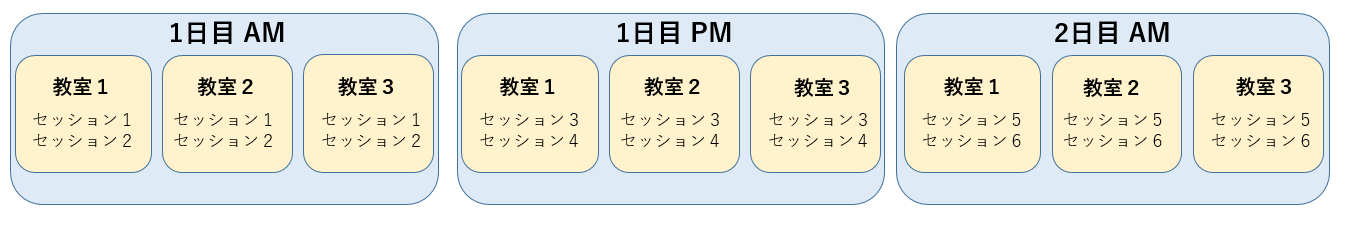
\includegraphics[scale=0.6]{gaiyou.png}
    \caption{特別研究報告審査会におけるセッションの構成}
    \label{Session}
  \end{center}
\end{figure}

この審査会のスケジュールは,従来,教員が手作業で作成していた.このスケジュールの作成には考慮すべき様々な条件がある.例えば,
\begin{itemize}
\item 学生は,自分自身と所属する研究室の教員が共に参加可能なセッションで発表する
\item 研究室が同じ学生は,教室をまたいで同時刻のセッションで発表しない
\item 各研究室は $1$ 日目AM,$1$ 日目PM,$2$ 日目AM のそれぞれで発表するのが望ましい
\end{itemize}
などの条件を考慮しなくてはならない.教員は,このような条件を考慮しながら,スケジュールを作成していた.しかし,これには大変な手間と時間を要していた.

そこで昨年度,本研究室での特別研究として,若林\cite{wakabayasi}は特別研究報告審査会のスケジュール作成自動化についての研究を行った.この研究では,スケジュール作成を最適化問題として定式化し,それを最適化ソルバを用いて解くことで,最適なスケジュールを得る手法を提案した.また,各研究室から情報を収集して最適化計算を行い,得られたスケジュールを PDF ファイルとして出力するインターフェースを開発した.昨年度の特別研究報告審査会は,実際にこの研究で作成されたスケジュールの下実施された.

しかし,\cite{wakabayasi}では,検討すべき事項として以下のことが挙げられていた.
\begin{itemize}
\item 期日にデータが揃わない
\item 研究室によって記入方法が異なっている\\
  各研究室から研究室,教員,学生,セッションの指定についての情報を記載した Excel ファイルを提出して頂いた.しかし研究室によってこのファイルへの記入方法は大きく異なっていたため, Excel ファイルの一部を手動で修正した.
  \begin{itemize}
  \item 教員名\\
    教員名は「姓+名」と記述する研究室と「姓+先生」と記述する研究室があったため「姓+名」という表記で統一した.
  \item 姓と名の間隔\\
    教員名,学生ともに姓名の間に半角あるいは全角でスペースを入れる研究室とスペースを入れない研究室に分かれていた.そのため,ここでは全角スペースで統一することとした.
  \item 学籍番号\\
    学籍番号は数字を半角入力する研究室と全角入力する研究室に分かれた.また,学籍番号の頭に $0$ をつけ桁数を統一する研究室があった(例:都$01$-$0001$).
  \end{itemize}
\item 特殊な希望がある教員,学生がいる\\
  特定の時間帯や,セッションの最後で発表することを希望する学生がいた.そこで,特定の時間帯で希望する学生についてはセッションの指定を行った.また,セッションの最後で発表することを希望する学生については,それぞれのセッションの中での発表順は公平を期すためにランダムにしているため,スケジュールを自動で作成した後に手動にて一部変更を行った.
\item 卒業論文のタイトルが長く,一覧表に $1$ 行で収まらない\\
  タイトルの長さは研究によって大きく異なり,一覧表に $1$ 行で収まらない学生がいた.そのため,収まらない学生のタイトルは手動により $2$ 行に変更した.
\item 作成したスケジュールに対して要望が発生した\\
  「ある研究室の発表を聞きたいので発表の時間をずらしてほしい」という要望が複数の研究室から発生した.そのため,手動により一部セッション内での発表順序を入れ替えるという変更を行った.
\end{itemize}

さらに,今年度,教員に対し特別研究報告審査会のスケジュールに関するアンケートを実施したところ,ある教員から「研究内容が近い研究室の教員が,お互いの研究室の発表を聞けるようにしてほしい」という要望を頂いた.

そこで本研究では,昨年度の研究で挙げられた検討事項の改良と,新たに発生した要望の実現を行う.具体的には以下の改良を行う.
\begin{itemize}
\item スケジュール作成問題の改良\\
昨年度作成された最適化モデルを改良し,頂いた要望を実現するために以下の$2$種類の制約条件を作成した.
\begin{itemize}
\item 関心度が高い研究室に所属する学生同士の発表順番が重複しない
\item 関心度が高い研究室同士の発表セッションが重複しない
\end{itemize}
\item インターフェースの利便性向上\\
研究室データを入力する Excel ファイルへの記入方法を以下のように改良した.
\begin{itemize}
\item 研究室名\\
研究室名は,研究室名のみを記述するように統一し,ドロップダウンメニューから選択するように改良した.
\item 教員名\\
教員名は「姓+名」に統一し,ドロップダウンメニューから選択するように改良した.
\item 姓と名の間隔\\
教員名,学生ともに姓名の間に全角でスペースを入れるように統一した.教員名はドロップダウンメニューから選択するように改良し,学生の氏名は,学籍番号を入力すると,その学籍番号に対応した学生の氏名が自動で入力されるように改良した.
\item 学籍番号\\
学籍番号は数字を半角入力するように統一した.また,学籍番号の桁数は $6$ 桁に統一し,ドロップダウンメニューから選択するように改良した(例:都 01-0001 ).
\end{itemize}
\end{itemize}

本研究で行った,最適化モデルの改良と,インターフェースの利便性向上については\ref{sec:model4}章と\ref{sec:inter}章にて記述する.
%%%%%%%%%%%%%%%%%%%%%%%%%%%%%%%%%%%%%%%%%%%%%%%%%%%%%%%%%%%%%%%%%%%%%
\newpage
\section{スケジュール作成問題の定式化の改良}\label{sec:model4}
本章では,昨年度作成された特別研究報告審査会のスケジュール作成問題の改良を行う.

今年度,教員に対し特別研究報告審査会のスケジュールに関するアンケートを実施したところ,ある教員から「研究内容が近い研究室の教員が,お互いの研究室の発表を聞けるようにしてほしい」という要望があった.そこで本研究では,この要望を実現するために,表\ref{tb:models}のような制約条件を追加した$2$種類のモデルを作成した.
\begin{table}[H]
  \begin{center}
    \caption{作成した$2$つのモデルと追加した制約条件}
    \label{tb:models}
    \begin{tabular}{c|p{13cm}} \toprule
    モデル名 & 追加した制約条件 \\ \bottomrule
    モデル$1$ & 関心度が高く発表を聞きに行きたい研究室に所属する学生同士の発表順番が重複しない\\
    モデル$2$ & 関心度が高く発表を聞きに行きたい研究室同士の発表セッションが重複しない\\ \bottomrule
    \end{tabular}
  \end{center}
 \end{table}

しかし,モデル$1$に追加した制約条件を表現するには,昨年度におけるモデルの添字付けでは不十分であった.具体的には,昨年度のモデルは発表セッションと発表教室のみを考慮していたが,モデル$1$に追加した制約条件を表現するためには学生の発表順番についても考慮する必要があった.そこで本研究では,昨年度のモデルに対し添字の変更を行い,新たな制約条件を追加したモデルを作成した.添字の変更を行った最適化モデルの内容と,新たに追加した制約条件の内容については,\ref{sec:model}節と\ref{sec:tuika}節にて記述する.また,添字の変更や新たな制約条件の追加を行ったため,目的関数にも変更を加えた.目的関数の変更点については\ref{sec:mokuteki}節にて記述する.


 \subsection{添字の変更を行った最適化モデル}\label{sec:model}
本節では,本研究で行った,最適化モデルの添字の変更について記述する.

本研究では,スケジュール作成問題を重み付き制約充足問題として扱っている.そのため,必ず満たさなければならない条件を絶対制約として扱い,できる限り満たしたい条件を考慮制約として扱う.ただし,本研究で作成した最適化モデルは,昨年度作成された最適化モデルから引用している.

まず,定式化に用いる集合・添字,パラメータ,変数について説明する.
\begin{itemize}
\item 集合・添字
  \begin{itemize}
  \item $d \in D$ :セッションを実施する時間帯とその集合
  \item $s \in S$ :セッションとその集合
  \item $f \in F_d$ :時間帯 $d$ でのセッション $s$ の組合せとその集合
  \item $a \in A_s$ :セッション $s$ での発表順番とその集合
  \item $r \in R$ :セッションを実施する教室とその集合
  \item $l \in L$ :研究室とその集合
  \item $i \in I$ :発表する学生とその集合
  \item $(l_1,l_2) \in O$ :一体運用している研究室の組合せとその集合
  \end{itemize}
\item パラメータ
  \begin{itemize}
  \item $u_{s}$ :セッション $s$ の発表人数の上限
  \item $m_{s,i}$ :学生のセッションへの参加可能性
    \begin{align*}
      \hspace{-0.3cm} m_{s,i} =
      \begin{cases}
	1, & \text{学生 $i$ はセッション $s$ に参加可能}\\
	0, & \text{学生 $i$ はセッション $s$ に参加不可能}
      \end{cases}
    \end{align*}
  \item $n_{s,l}$ :教員のセッションへの参加可能性
    \begin{align*}
      \hspace{-0.3cm} n_{s,l} =
      \begin{cases}
	1, & \text{研究室 $l$ の教員はセッション $s$ に参加可能}\\
	0, & \text{研究室 $l$ の教員はセッション $s$ に参加不可能}
      \end{cases}
    \end{align*}
  \item $b_{l,i}$ :学生の研究室への所属関係
    \begin{align*}
      \hspace{-0.3cm} b_{l,i} =
      \begin{cases}
	1, & \text{学生 $i$ が研究室 $l$ に所属している} \\
	0, & \text{学生 $i$ が研究室 $l$ に所属していない}
      \end{cases}
    \end{align*}
  \end{itemize}
\item 変数
  \begin{itemize}
  \item $x_{s,r,i,a}$ :学生の発表を表す $0\mathchar`-1$ 変数
    \begin{align*}
      \hspace{-0.3cm} x_{s,r,i,a} =
      \begin{cases}
	1, & \text{学生 $i$ がセッション $s$,部屋 $r$,発表順番 $a$ で発表する} \\
	0, & \text{学生 $i$ がセッション $s$,部屋 $r$,発表順番 $a$ で発表しない}
      \end{cases}
    \end{align*}
  \item $y_{s,r,l}$ :指定された研究室に所属する学生の発表を表す $0\mathchar`-1$ 変数
    \begin{align*} 
      \hspace{-0.3cm} y_{s,r,l} = 
      \begin{cases}
	1, & \text{研究室 $l$ の学生がセッション $s$,部屋 $r$ で発表する} \\
	0, & \text{研究室 $l$ の学生がセッション $s$,部屋 $r$ で発表しない}
      \end{cases}
    \end{align*}
  \item $v_{s,r}$ :セッション $s$,部屋 $r$ での発表人数
  \item $w_{d,l}$ :研究室 $l$ に所属する学生の時間帯 $d$ の発表人数
  \item $z_{s,r,l}$ :教員の司会担当を表す $0\mathchar`-1$ 変数
    \begin{align*} 
      \hspace{-0.3cm} z_{s,r,l} = 
      \begin{cases}
	1, & \text{研究室 $l$ の教員がセッション $s$,部屋 $r$ で司会をする}\\
	0, & \text{研究室 $l$ の教員がセッション $s$,部屋 $r$ で司会をしない}
      \end{cases}
    \end{align*}
  \item $p_{1,s}$ :考慮制約 $1$(後述)における違反の有無
  \item $p_{2,d,l}$ :考慮制約 $2$(後述)における違反の有無
  \item $p_{3,d,d,l}$ :考慮制約 $3$(後述) における違反量
  \item $p_{4,i_1,i_2}$ :考慮制約 $4$(後述) における違反の有無\\

  ただし
\begin{align*}
      \hspace{-0.3cm} p_{1,s}, \quad p_{2,d,l}, \quad p_{4,i_1,i_2} = %% \quad p_{5,l_1,l_2}
      \begin{cases}
	1, & \text{考慮制約に違反している}\\
	0, & \text{考慮制約に違反していない}
      \end{cases}
    \end{align*}
    である.
  \end{itemize}
\end{itemize}

 次に,絶対制約について記述する.
 \begin{description}
\item[絶対制約 $1$] 全学生が $1$ 回ずつ発表する.\\発表しない学生,あるいは複数回発表する学生が存在してはならない.全ての学生 $i$ がいずれかのセッション $s$,部屋 $r$ で $1$ 回だけ発表することを表すために
  \begin{eqnarray}
    \sum_{s \in S, r \in R, a \in A_s} x_{s,r,i,a} = 1 \quad (i \in I)
  \end{eqnarray}
  という制約を設ける.
\item[絶対制約 $2$] 学生は,自分自身と研究室の教員が共に参加可能なセッションで発表する.\\各研究室からは,所属学生と担当教員が参加不可能なセッションの情報を収集する.この情報を元に,学生自身および研究室の担当教員が共に参加可能なセッションで各学生が発表するために
  \begin{eqnarray}
    x_{s,r,i,a} \leq m_{s,i}  n_{s,l} \quad (s \in S, r \in R, l \in L, i \in I , a \in A_s , b_{l,i}=1) \label{eq:Const2}
  \end{eqnarray}
  という制約を設ける.(\ref{eq:Const2}) の右辺は,$m_{s,i} = n_{s,l} = 1$ のとき,すなわち学生・担当教員が共に参加可能なときのみ $1$ となる.このとき (\ref{eq:Const2}) は
  \begin{eqnarray*}
    x_{s,r,i,a} \leq 1 \quad (s \in S, r \in R, l \in L, i \in I , a \in A_s , b_{l,i}=1)
  \end{eqnarray*}
  となり,学生 $i$ がセッション $s$,部屋 $r$,発表順番 $a$ で発表することが可能になる.一方これ以外のとき,すなわち学生・担当教員のどちらか(あるいは両方)が参加不可能であるとき (\ref{eq:Const2}) は
  \begin{eqnarray*}
    x_{s,r,i,a} \leq 0 \quad (s \in S, r \in R, l \in L, i \in I , a \in A_s , b_{l,i}=1)
  \end{eqnarray*}
  となり,$x_{s,r,i,a}$ が $0\mathchar`-1$ 変数であることから $x_{s,r,i,a} = 0$となるため, 学生 $i$ がセッション $s$,部屋 $r$,発表順番 $a$ で発表することが不可能になる.
\item[絶対制約 $3$] 各研究室は複数のセッションで発表する.\\$1$ つのセッションだけで全員が発表を終えてしまう研究室が存在するのは良い状態ではない.同じ研究室の学生による発表が偏ることを防ぐために
  \begin{eqnarray}
    \sum_{s \in S, r \in R} y_{s,r,l} \geq 2 \quad (l \in L)
  \end{eqnarray}
  という制約を設ける.
\item[絶対制約 $4$] 研究室が同じ学生は,教室をまたいで同時刻のセッションで発表しない.\\同時刻に開催しているセッションで教室をまたいで発表する研究室があると,その研究室の教員が担当学生の発表を確認できない可能性がある.よって,これを防ぐために
  \begin{eqnarray}
    \sum_{r \in R} y_{s,r,l} \leq 1 \quad (s \in S, l \in L)
  \end{eqnarray}
  という制約を設ける.
\item[絶対制約 $5$] 学生個人の発表と,指定された研究室に所属する学生の発表が対応する.\\本問題の定式化に際しては,学生 $i$ という個人の発表と,指定された研究室 $l$ に所属する学生(学生個人は特定しない)の発表を分けて考えている.学生個人 $i$ の発表の有無と研究室 $l$ に所属する学生の発表の有無には,以下の関係がある.
  \begin{itemize}
  \item 研究室 $l$ に所属する学生の発表がないとき,その研究室に所属する学生 $i$ は誰も発表することができない
  \item 研究室 $l$ に所属する学生の発表があるとき,その研究室に所属する学生 $i$ は発表してもしなくてもよい
  \item 研究室 $l$ に所属する学生の発表があるとき,その研究室に所属する学生 $i$ は少なくとも誰か$1$人は発表しなければならない
  \end{itemize}
  これらの関係を表すために
  \begin{eqnarray}
   \sum_{a \in A_s} x_{s,r,i,a} & \leq & y_{s,r,l} \quad (s \in S, r \in R, l \in L, i \in I, b_{l,i} = 1) \label{eq:Const5_1} \\
    y_{s,r,l} & \leq & \sum_{i \in I, a \in A_s} x_{s,r,i,a} \quad (s \in S, r \in R, l \in L, b_{l,i} = 1) \label{eq:Const5_2}
  \end{eqnarray}
  という $2$ つの制約を設ける.$y_{s,r,l}=0$ のとき,すなわち研究室 $l$ に所属する学生の発表がないときは,(\ref{eq:Const5_1}) より
  \begin{eqnarray*}
   \sum_{a \in A_s} x_{s,r,i,a} \leq 0 \quad (s \in S, r \in R, l \in L, i \in I, b_{l,i} = 1)
  \end{eqnarray*}
  となり,$x_{s,r,i,a}$ が $0\mathchar`-1$ 変数であることから $x_{s,r,i,a} = 0$ となるため,研究室 $l$ に所属する学生 $i$ は誰も発表することができない.一方$y_{s,r,l}=1$ のとき,すなわち研究室 $l$ に所属する学生の発表があるときは,(\ref{eq:Const5_1}), (\ref{eq:Const5_2}) は
  \begin{eqnarray*}
    x_{s,r,i,a} \leq 1 \leq \sum_{i \in I, a \in A_s} x_{s,r,i,a} \quad (s \in S, r \in R, l \in L, b_{l,i} = 1)
  \end{eqnarray*}
  となり,$0\mathchar`-1$ 変数 $x_{s,r,i,a}$ は値が $1$ になることができ,かつ研究室 $l$ に所属する学生 $i$ が $1$ 人以上発表することになる.
\item[絶対制約 $6$] 一体運用を行う研究室は同じセッションにて発表する.\\研究室が異なっていても,研究の類似性・関連性から一体運用を行っている研究室が存在する.そのような研究室の発表は同じセッションで行いたい.そのため
  \begin{eqnarray}
    y_{s,r,l_1} = y_{s,r,l_2} \quad(s \in S, r \in R, (l_1, l_2) \in O)
  \end{eqnarray}
  という制約を設ける.
\item[絶対制約 $7$] 各セッションの発表人数の計算.\\各セッションの発表人数を計算するために
  \begin{eqnarray}
    v_{s,r} = \sum_{i \in I, a \in A_s} x_{s,r,i,a} \quad (s \in S, r \in R)
  \end{eqnarray}
  という制約を設ける.本制約で求めた各セッションの発表人数は考慮制約で使用する.
\item[絶対制約 $8$] 各セッションの発表者数は上限を超えない.\\時間の都合やセッション毎の発表人数のバランスにより,セッション毎に発表できる人数には限りがある.各セッションの発表者数が上限を超えないことを表すために
  \begin{eqnarray}
    v_{s,r} \leq u_{s} \quad (s \in S, r \in R)
  \end{eqnarray}
  という制約を設ける.
\item[絶対制約 $9$] 研究室の日程毎の発表者数の計算.\\各研究室の日程毎の発表者数を計算するために
  \begin{eqnarray}
    w_{d,l} = \sum_{f \in F_d, r \in R, i \in I, a \in A_s} x_{f,r,i,a} \quad (d \in D, l \in L, b_{l,i} = 1) \label{eq:Const9}
  \end{eqnarray}
  という制約を設ける.$f$ は,日程 $d$ で行われるセッション $s$ の組合せであるから,(\ref{eq:Const9}) の右辺は各日程で行われるセッションの発表人数の合計となる.
  本制約で求めた研究室の日程毎の発表者数は考慮制約で使用する.
\item[絶対制約 $10$] 全セッションで教員が司会をする.\\発表を滞りなく進めていくために,全てのセッションで教員による司会進行が必要となる.そのため
  \begin{eqnarray}\sum_{l \in L} z_{s,r,l} = 1 \quad (s \in S, r \in R)
  \end{eqnarray}
  という制約を設ける.
\item[絶対制約 $11$] 研究室での発表がある場合,その研究室の教員が司会をすることがある.\\教員が司会をすることがあるのは,教員が指導する研究室の学生が発表するセッションであるものとする.これを表すために
  \begin{eqnarray}z_{s,r,l} \leq y_{s,r,l} \quad (s \in S, r \in R, l \in L) \label{eq:Const11}
  \end{eqnarray}
  という制約を設ける.$y_{s,r,l}=1$ のとき,すなわち研究室の発表があるとき(\ref{eq:Const11}) は
  \begin{eqnarray*}
    z_{s,r,l} \leq 1 \quad (s \in S, r \in R, l \in L)
  \end{eqnarray*}
  となり,研究室 $l$ の教員はセッション $s$,部屋 $r$ で司会をすることが可能になる.
\item[絶対制約 $12$] 各教員が司会をするのは $1$ 度まで.\\特定の研究室の教員に司会の負担を集中させるのは良い状態とは言えない.研究室数はセッション数よりも多いため,研究室毎に教員が司会をするのは $1$ 度までとすることができる.これを表すために
  \begin{eqnarray}
    \sum_{s \in S, r \in R} z_{s,r,l} \leq 1 \quad (l \in L)
  \end{eqnarray}
  という制約を設ける.

 次に,考慮制約について記述する.\\
\item[考慮制約 $1$] 同時刻に行われているセッションにおいて,発表人数の最大と最小の差は $1$ 以下とする.\\同時刻にはそれぞれのセッションで $3$ 部屋で並行して発表が行われているが,$1$ つの部屋だけ早く終わったり,遅くまで行われている状態は避けたい.そのため,同時刻に開催するセッションの発表人数は等しくしたい.しかし,発表人数が部屋数で割り切れるとは限らず,同時刻に開催するセッションの発表人数は等しくできないことがある.そのため
  \begin{eqnarray}
    v_{s,r_1} - v_{s,r_2} \leq p_{1,s} \quad (s \in S, r_1 \in R, r_2 \in R,  r_1 \neq r_2)
  \end{eqnarray}
  という制約を設ける.違反変数 $p_1$ は $0\mathchar`-1$ 変数であるため,$3$ 部屋での発表人数はできる限り等しくなる.
\item[考慮制約 $2$] 各研究室は全ての日程で発表するのが望ましい.\\全ての日程 $d$($1$ 日目AM,$1$ 日目PM,$2$ 日目AM)で各研究室ができる限り発表するために
  \begin{eqnarray}
    -p_{2,d,l} \leq \sum_{r \in R, f \in F_d} y_{f,r,l} - 1 \leq p_{2,d,l} \quad (d \in D, l \in L) \label{eq:p2}
    %\left| \sum_{r \in R} (y_{d,s_1,r,l} + y_{d,s_2,r,l}) - 1 \right| \leq p_{2,d,l}
  \end{eqnarray}
  という制約を設ける.ここで(\ref{eq:p2}) の中央の式について説明する.まず,$y$ の添字である $f$ は,日程 $d$ に開催されているセッション,つまりセッション $1$ と $2$,$3$ と $4$,$5$ と $6$ の組合せのことであり,和を計算している部分は $1$ 日目AM,$1$ 日目PM,$2$ 日目AM のそれぞれでの発表セッション数を表している.よって
  \begin{itemize}
  \item $s_1$, $s_2$ のどちらも発表しないとき \quad $\displaystyle \sum_{f \in F,r \in R} (y_{f_1,r,l} + y_{f_2,r,l}) = 0$
  \item $s_1$, $s_2$ のどちらかで発表するとき \quad $\displaystyle \sum_{f \in F,r \in R} (y_{f_1,r,l} + y_{f_2,r,l}) = 1$
  \item $s_1$, $s_2$ のどちらも発表するとき \qquad $\displaystyle \sum_{f \in F,r \in R} (y_{f_1,r,l} + y_{f_2,r,l}) = 2$
  \end{itemize}
  となる.この総和部分の値から $1$ を引くため,$s_1$, $s_2$ のどちらかで発表するときのみ (\ref{eq:p2}) は 
  \begin{eqnarray*}
    -p_{2,d,l} \leq 0 \leq p_{2,d,l}
  \end{eqnarray*}
  となり,違反の有無を表す変数 $p_2$ は値 $0$ をとることができる.
\item[考慮制約 $3$] 各研究室の中で,日程毎の発表者数の差は少ない状態が望ましい.\\考慮制約 $2$ によって,$1$ 日目AM,$1$ 日目PM,$2$ 日目AM のそれぞれで発表したとしても,その人数が偏っている状態は避けたい.つまり,日程毎の発表者数はできる限り等しくしたい.しかし,研究室の人数が日程の数で割り切れるとは限らず,日程の発表者数は等しくできないことがある.そのため
  \begin{eqnarray}
    -p_{3,d_1,d_2,l} \leq w_{d_1,l} - w_{d_2,l} \leq p_{3,d_1,d_2,l} \quad (d_1 \in D, d_2 \in D, l \in L, d_1 \neq d_2)
    %\left| w_{d_1,l} - w_{d_2,l} \right| \leq p3_{d_1,d_2,l}
  \end{eqnarray}
  という制約を設ける.
\item[考慮制約 $4$] 同じセッションで発表するのが望ましい学生の組合せをできるだけ成立させる.\\研究内容に関連性や類似性のある学生は,研究室にかかわらずできる限り同じセッションで発表するのが望ましい.これを表すために
  \begin{eqnarray}
    -p_{4,i_1,i_2} \leq \sum_{a \in A_s} x_{s,r,i_1,a} - \sum_{a \in A_s}x_{s,r,i_2,a} \leq p_{4,i_1,i_2} \quad (s \in S, r \in R, (i_1, i_2) \in C)
  \end{eqnarray}
  という制約を設ける.
    \end{description}

\subsection{追加した制約条件の内容}\label{sec:tuika}
本節では,頂いた要望を実現するために新たに作成した $2$ 種類の制約条件について説明する.

頂いた要望は「研究内容が近い研究室の教員が,お互いの研究室の発表を聞けるようにしてほしい」という内容であった.この要望を実現するために,新たに$2$ 種類の制約条件を作成し,考慮制約として定式化を行った.

まず $1$ つ目の制約条件について説明する.$1$ つ目の制約条件は「関心度が高く発表を聞きに行きたい研究室があった場合,その研究室に所属する学生同士の発表順番ができるだけ重複しないことが望ましい」という内容である.

昨年度の最適化モデルでは,発表順番については考慮しておらず,発表セッションと発表教室のみを考慮していた.そのため,次の例のような問題が発生する可能性があった:例として,研究室 $A$ の教員が,研究室 $B$ の学生の発表を聞きたい場合を考える.仮に,スケジュールが図 \ref{fig:Before} のようなものであった場合,教員 $A$ は,自分の担当する研究室 $A$ の学生の発表を聞く必要があるため,教室 $1$ にいる必要がある.しかし,研究室$B$の学生が,教室$3$で,研究室$A$の学生と同じ発表順番で発表を行っているため,教員 $A$ は,研究室 $B$ の学生の発表を聞きに行くことができない.
\begin{figure}[H]
  \begin{center}
    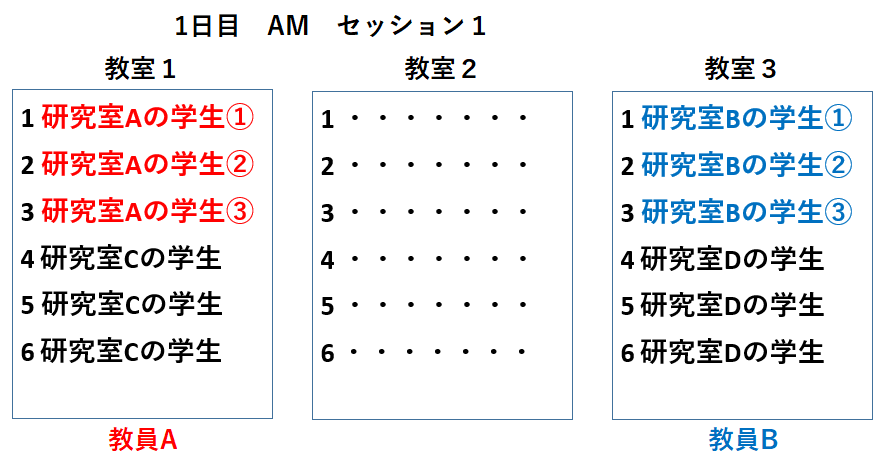
\includegraphics[scale=0.65]{BeforeOrder.png}
    \caption{発表順番を考慮していないスケジュール}
    \label{fig:Before}
  \end{center}
\end{figure}
しかし,発表順番を考慮し,スケジュールを図 \ref{fig:after} のように変更すると,教員 $A$ は,自分の担当する学生の発表が終わり次第教室を移動し,研究室 $B$ の学生の発表を聞きに行くことが可能になる.
\begin{figure}[H]
  \begin{center}
    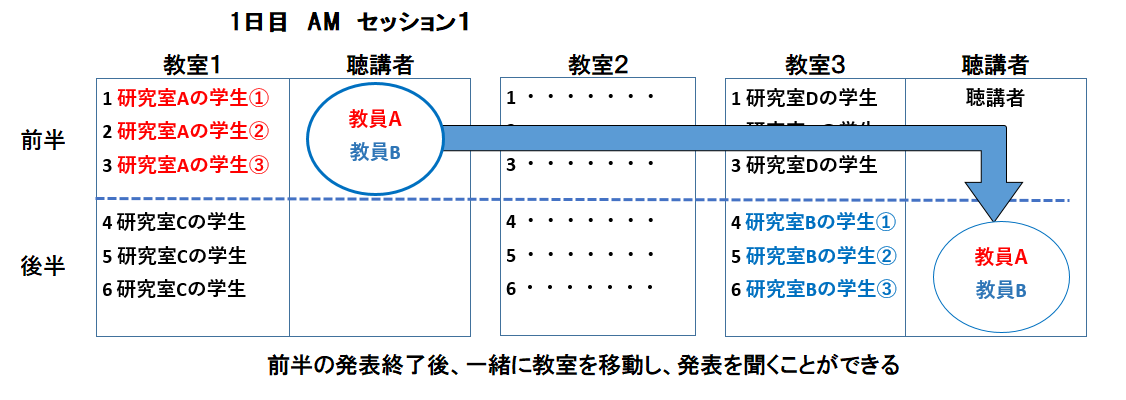
\includegraphics[scale=0.65]{AfterOrder.png}
    \caption{発表順番を考慮したスケジュール}
    \label{fig:after}
  \end{center}
\end{figure}
この状態を実現するために,以下の考慮制約 $5\mathchar`-1$ を作成した.
 \begin{description}
\item[考慮制約 $5\mathchar`-1$] 関心度が高く発表を聞きたい研究室があった場合,その研究室に所属する学生同士の発表順番ができるだけ重複しないことが望ましい
  \begin{eqnarray}
   \sum_{r \in R} (x_{s,r,i_1,a} + x_{s,r,i_2,a}) - 1 \leq p_{5,l_1,l_2} \label{eq:p5}
  \end{eqnarray}
  \begin{center}
  $(s \in S,a \in A_s,i_1 \in I,i_2 \in I,(l_1,l_2) \in G,b_{l_1,i_1} = 1,b_{l_2,i_2} = 1)$
  \end{center}
  \end{description}
  
一方,この制約条件には,発表を聞きたい研究室の組合せが多くなると,セッション内での教室移動の回数が多くなる可能性があった.そこで,次の $2$ つ目の制約条件として,学生の発表順番ではなく,研究室の発表セッションができるだけ重複しないような制約条件を作成した.

$2$ つ目の制約条件は「関心度が高く発表を聞きたい研究室があった場合,その研究室同士の発表セッションができるだけ重複しないことが望ましい」という内容である.先ほどの例と同じように,研究室 $A$ の教員が,研究室 $B$ の学生の発表を聞きたい場合を考える.仮にスケジュールが図 \ref{fig:befor2} のようなものであった場合,研究室 $A$ と研究室 $B$ の発表セッションが重複しているため,図 \ref{fig:Before} と同様に学生の発表順番が重複する可能性がある.
\begin{figure}[H]
  \begin{center}
    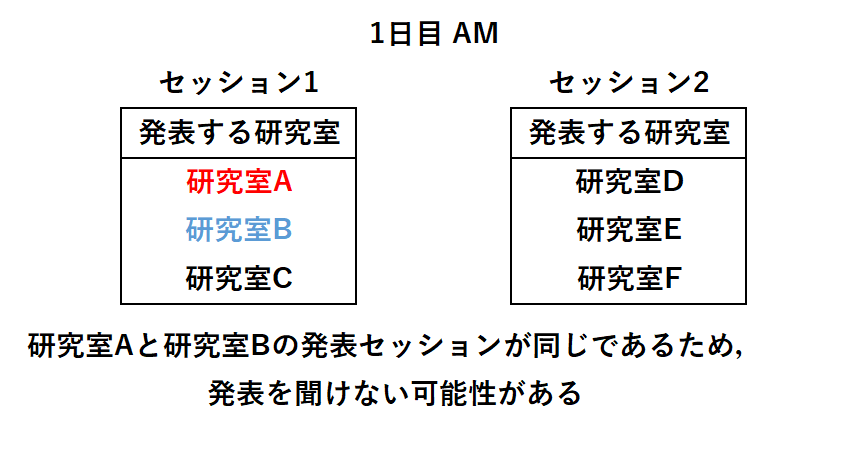
\includegraphics[scale=0.65]{befor2.png}
    \caption{発表セッションが重複しているスケジュール}
    \label{fig:befor2}
  \end{center}
\end{figure}
しかし,$2$ つの研究室の発表セッションが重複しないよう,スケジュールを図 \ref{fig:after2} のように変更すると,教員 $A$ は,自分の担当する研究室の発表セッション終了後,研究室 $B$ の学生が発表するセッションに参加し,発表を聞くことが可能になる.
\begin{figure}[H]
  \begin{center}
    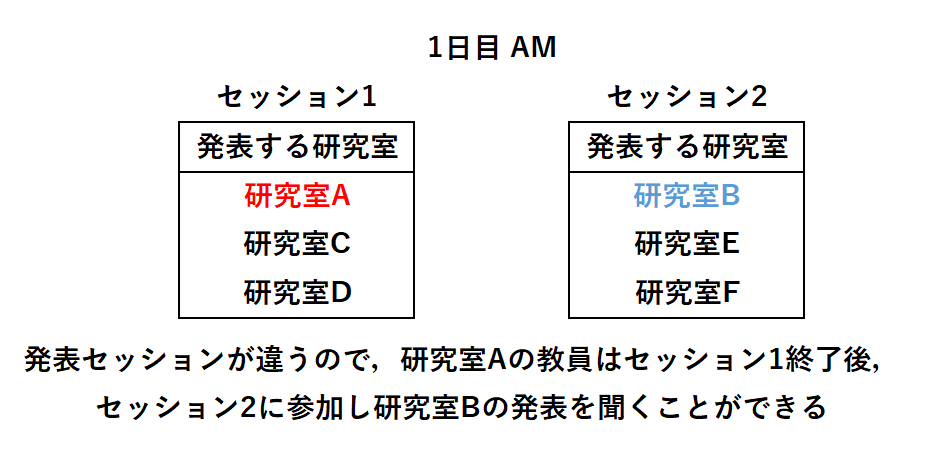
\includegraphics[scale=0.65]{after2.png}
    \caption{発表セッションが重複していないスケジュール}
    \label{fig:after2}
  \end{center}
\end{figure}
この状態を実現するために,次の考慮制約 $5\mathchar`-2$ を作成した.
 \begin{description}
 \item[考慮制約 $5\mathchar`-2$] 関心度が高く発表を聞きたい研究室があった場合,その研究室同士の発表セッションができるだけ重複しないことが望ましい
   \begin{eqnarray}
    \sum_{r \in R} (y_{s,r,l_1} + y_{s,r,l_2}) - 1 \leq p_{5,l_1,l_2} \quad (s \in S,(i_1,i_2) \in G) \label{eq:p6}
  \end{eqnarray}
  \end{description}
以上が,本研究で新たに作成した$2$つの制約条件の内容である.

\subsection{変更を行った目的関数}\label{sec:mokuteki}
本節では,本研究で変更を行った目的関数について記述する.

目的関数は,考慮制約 $1$, $2$, $3$, $4$, $5$の違反量または違反の有無を表す変数 $p_1$, $p_2$, $p_3$, $p_4$, $p_5$ の合計値に考慮制約の重要度を表す重み $w_1$, $w_2$, $w_3$, $w_4$, $w_5$ を乗じたものの和とする.具体的には以下のように表すことができる.
\begin{eqnarray}
  \text{minimize} &\quad& w_1 \cdot \sum_{d \in D, s \in S_d} p_{1,d,s} + w_2 \cdot \sum_{d \in D, l \in L} p_{2,d,l} + w_3 \cdot \sum_{d_1 \in D, d_2 \in D, l \in L} p_{3,d_1,d_2,l} \nonumber \\
  && + w_4 \cdot \sum_{(i_1, i_2) \in C} p_{4,i_1,i_2} + w_5 \cdot \sum_{(l1,l2) \in G} p_{5,l1,l2}
\end{eqnarray}

%%%%%%%%%%%%%%%%%%%%%%%%%%%%%%%%%%%%%%%%%%%%%%%%%%%%%%%%%%%%%%%%%%%%%%
\newpage
\section{インタフェースの利便性向上}\label{sec:inter}
本章では,本研究で行ったスケジュール作成を自動化するインターフェースの改良について記述する.

昨年度作成されたインターフェースには,以下のような修正すべき事項があった.
\begin{itemize}
\item 研究室データが記入された Excel ファイルへの記入方法が異なっていた
  \begin{itemize}
  \item 教員名\\
    教員名は「姓+名」と記述する研究室と「姓+先生」と記述する研究室があったため「姓+名」という表記で統一した.
  \item 姓と名の間隔\\
    教員名,学生ともに姓名の間に半角あるいは全角でスペースを入れる研究室とスペースを入れない研究室に分かれていた.そのため,ここでは全角スペースで統一することとした.
  \item 学籍番号\\
    学籍番号は数字を半角入力する研究室と全角入力する研究室に分かれた.また,学籍番号の頭に $0$ をつけ桁数を統一する研究室があった(例:都$01$-$0001$).
  \end{itemize}
\item インタフェースの利用環境が変わるたびに,バッチファイルを書き換える必要があった.
\end{itemize}
本研究では,これらの事項を改良し,インタフェースの利便性を向上した.

\subsection{Excel ファイルへの記入方法の改良}
本節では,本研究で行った Excel ファイルの記入方法の改良点について記述する.

昨年度は,特別研究報告審査会のスケジュールを作成するために,各研究室に図 \ref{fig:wakaexcel} のような研究室データを記入する Excel ファイルを配布し,提出して頂いた.
\begin{figure}[H]
  \begin{center}
    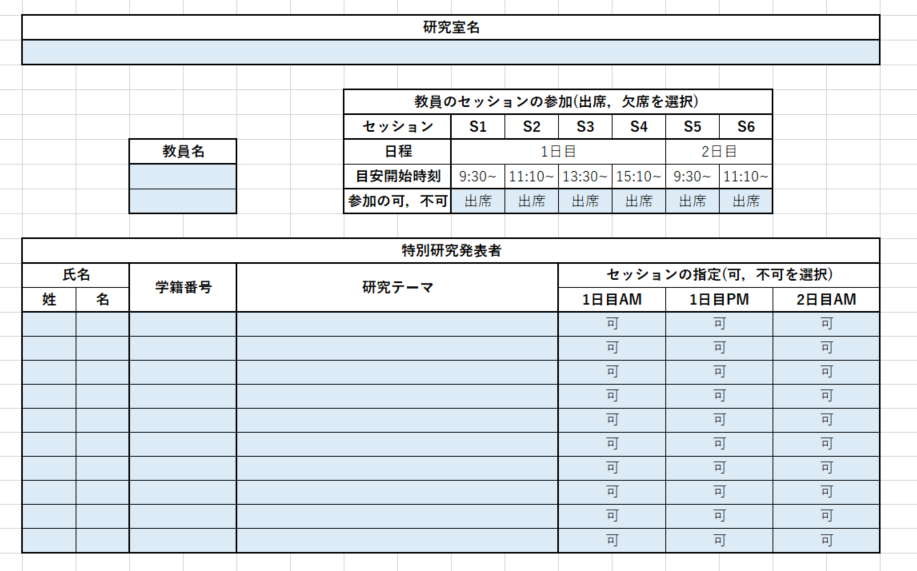
\includegraphics[scale=0.8]{wakaexcel.png}
    \caption{昨年度配布した Excel ファイル}
    \label{fig:wakaexcel}
  \end{center}
\end{figure}
しかし,研究室によって,この Excel ファイルへの記入方法が異なっており,ファイルの一部を手動で修正する必要があった.修正が必要であった点は,以下の $5$ 点である.
\begin{itemize}
\item 研究室名\\
研究室名は「研究室名+研究室」と記述する研究室と,研究室名のみを記述する研究室があった.
\item 研究室 ID\\
研究室を識別するための研究室 ID は,データを提出して頂いたあと,手動で入力した.
\item 教員名\\
教員名は「姓+名」と記述する研究室と「姓+先生」と記述する研究室があった.
\item 姓と名の間隔\\
教員名,学生ともに姓名の間に半角あるいは全角でスペースを入れる研究室と,スペースを入れない研究室に分かれていた.
\item 学籍番号\\
学籍番号は数字を半角入力する研究室と,全角入力する研究室に分かれた.また,学籍番号の頭に 0 をつけ桁数を統一する研究室があった(例:都 01-0001 ).
\end{itemize}

そこで,本研究では,Excel ファイルの記入方法を改良し,記入方法の統一を行った.改良内容は,以下の通りである.
\begin{itemize}
\item 研究室名\\
研究室名は,研究室名のみを記述するように統一し,ドロップダウンメニューから選択するように改良した.
\item 研究室 ID\\
研究室を識別するための研究室 ID は,研究室名を選択すると自動で入力されるように改良した.
\item 教員名\\
教員名は「姓+名」に統一し,ドロップダウンメニューから選択するように改良した.
\item 姓と名の間隔\\
教員名,学生ともに姓名の間に全角でスペースを入れるように統一した.教員名はドロップダウンメニューから選択するように改良し,学生の氏名は,学籍番号を選択すると,その学籍番号に対応した学生の氏名が自動で入力されるように改良した.
\item 学籍番号\\
学籍番号は数字を半角入力するように統一した.また,学籍番号の桁数は $6$ 桁に統一し,ドロップダウンメニューから選択するように改良した(例:都 01-0001 ).
\end{itemize}
\begin{figure}[H]
  \begin{center}
    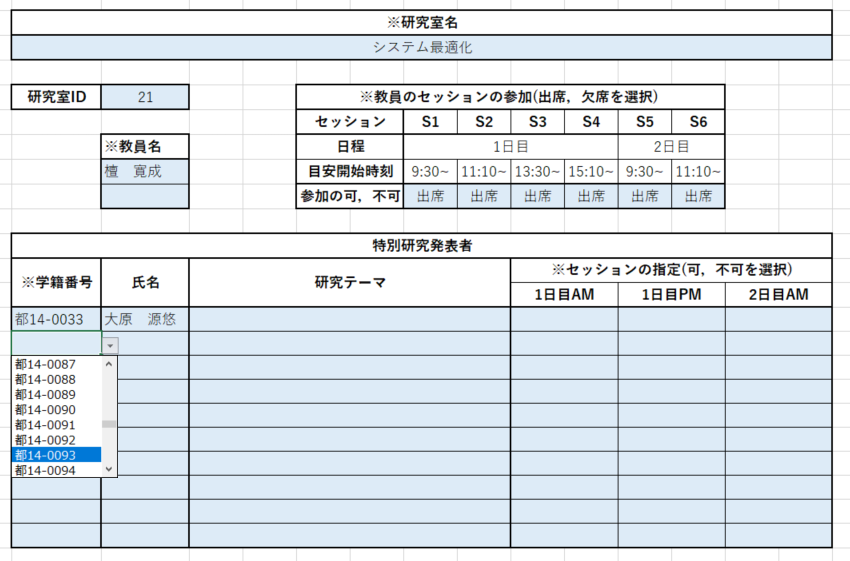
\includegraphics[scale=0.8]{dropdown.png}
    \caption{改良後の Excel ファイル}
    \label{fig:dropdown}
  \end{center}
\end{figure}

\subsection{バッチファイル自動作成機能の実装}
昨年度作成されたインターフェースでは,インタフェースの利用環境が変わるたび,図 \ref{fig:bat} のようなバッチファイルを書き換える必要があった.
\begin{figure}[H]
  \begin{center}
    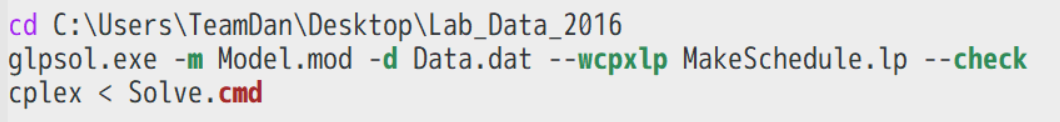
\includegraphics[scale=0.7]{bat.png}
    \caption{バッチファイル}
    \label{fig:bat}
  \end{center}
\end{figure}
しかし,このバッチファイルには,インタフェースを実行する上で重要なコマンドが記述されている.なので,インタフェースの利用環境が変わるたびにこのバッチファイルを書き換えていると,インタフェースの保守性が損なわれる可能性があった.そこで,本研究では,インターフェースを実行すると,図 \ref{fig:bat} のようなバッチファイルが自動で作成されるような機能を実装し,インタフェースの利用環境が変わってもバッチファイルの書き換えを行う必要がないように改良した.

\subsection{改良後の内部処理} \label{sec:InternalProcessing}
本節では,本研究で改良したインターフェースの内部処理について説明する.

まず,昨年度作成されたインターフェースの内部処理を図\ref{fig:wakac}に示す.
\begin{figure}[H]
  \begin{center}
    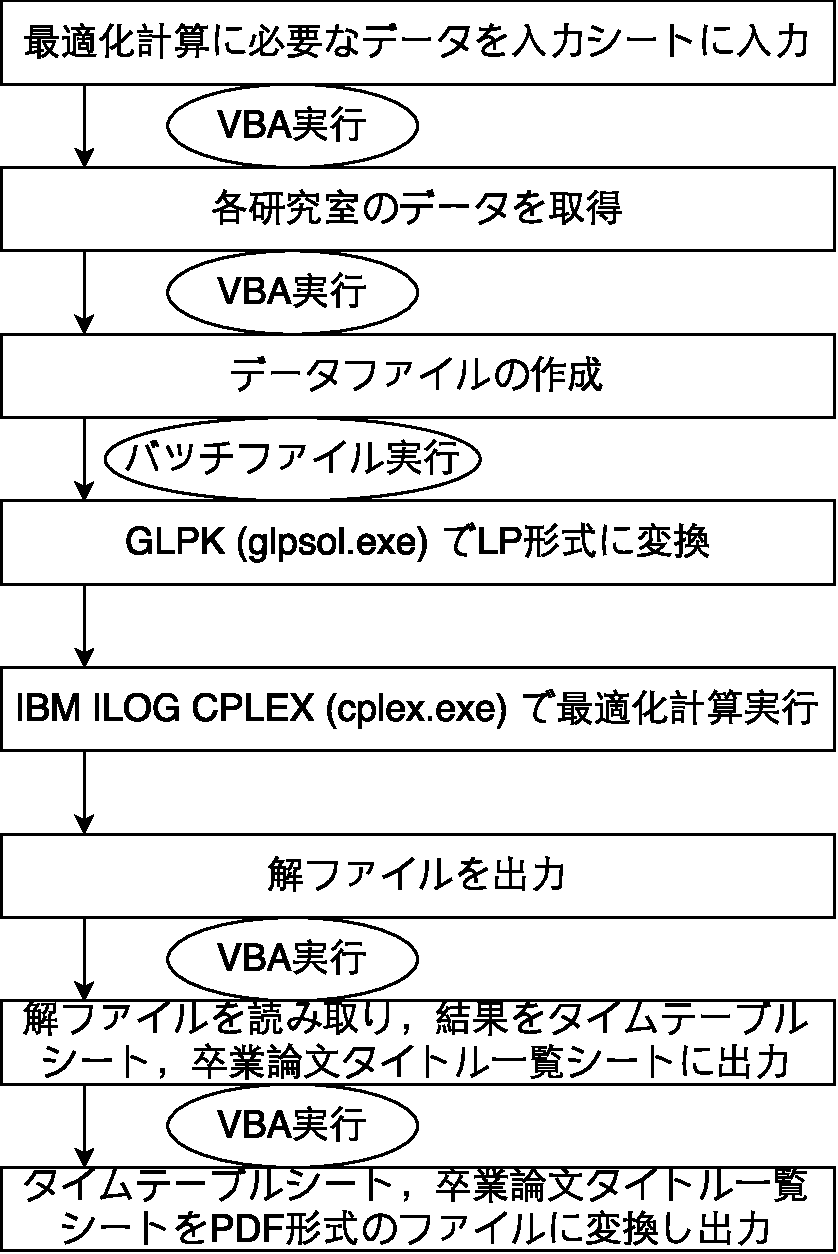
\includegraphics[scale=1.0]{fig_FlowChart.pdf}
    \caption{昨年度作成されたインターフェースの内部処理の手順}
    \label{fig:wakac}
  \end{center}
\end{figure}

本研究では,昨年度作成されたインターフェースに新たにバッチファイル自動作成の機能を追加した.そのため,インターフェースの内部処理も以下の図\ref{fig:FlowChart}のように変更した.
\begin{figure}[H]
  \begin{center}
    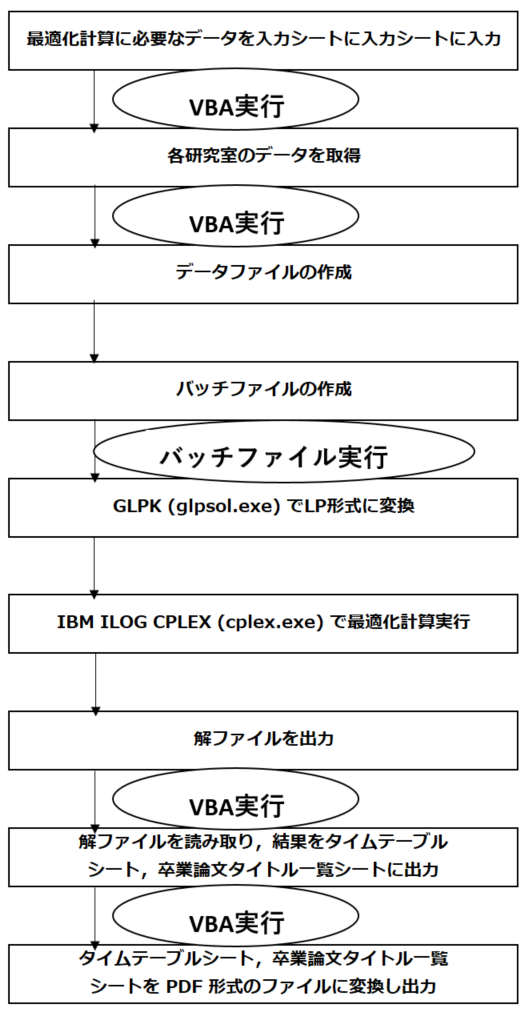
\includegraphics[scale=1.0]{FloxChart.png}
    \caption{今年度改良を行ったインターフェースの内部処理の手順}
    \label{fig:FlowChart}
  \end{center}
\end{figure}

\begin{flushleft} 以下,この内部処理について詳しく説明する.  \end{flushleft}


初めに,処理を行う準備として,手動により最適化計算に必要なデータおよびスケジュール一覧表を作成するのに必要なデータを,インターフェースの入力シート(図 \ref{fig:inter})に入力しておく必要がある.

 まず,プログラミング言語 VBA を用いて,各研究室に提出して頂いた,最適化計算に必要な各研究室の研究室名,研究室 ID,教員名,発表者の名前,学籍番号,テーマ,参加不可能なセッションの情報が入力された Excel ファイルを読み込む.このとき,インターフェースの入力シートに入力した絶対パスのフォルダ内のファイルを参照している.

次に,VBA を用いて,インターフェースの入力シートに入力した情報および Excel ファイルから取得した各研究室の情報を元に,最適化計算に用いる GMPL 形式のデータファイルを作成する.

次に,GMPL 形式であらかじめ作成されているモデルファイル (Model.mod) と,作成したデータファイル (Data.dat) を GLPK を用いて LP 形式のファイル (MakeSchedule.lp) に変換するためのバッチファイル (FileConvert.bat) を作成し,実行する.その後,作成された LP ファイルをコマンドファイル (Solve.cmd) を用いて CPLEX に読み込ませ,最適化計算を行う.最適化計算が終了すると,解ファイル (MakeSchedule.sol) が出力される.

最後に,VBA を用いて,最適化計算により得た解ファイルの情報を整理し,セッション毎,部屋毎の発表者の情報をタイムテーブルシート(図 \ref{fig:time})に出力する.また,同様に,解ファイルの情報を整理し,研究室毎に卒業論文のタイトルを発表順に卒業論文タイトル一覧シート(図 \ref{fig:title})に出力する.

\begin{figure}[H]
  \begin{center}
    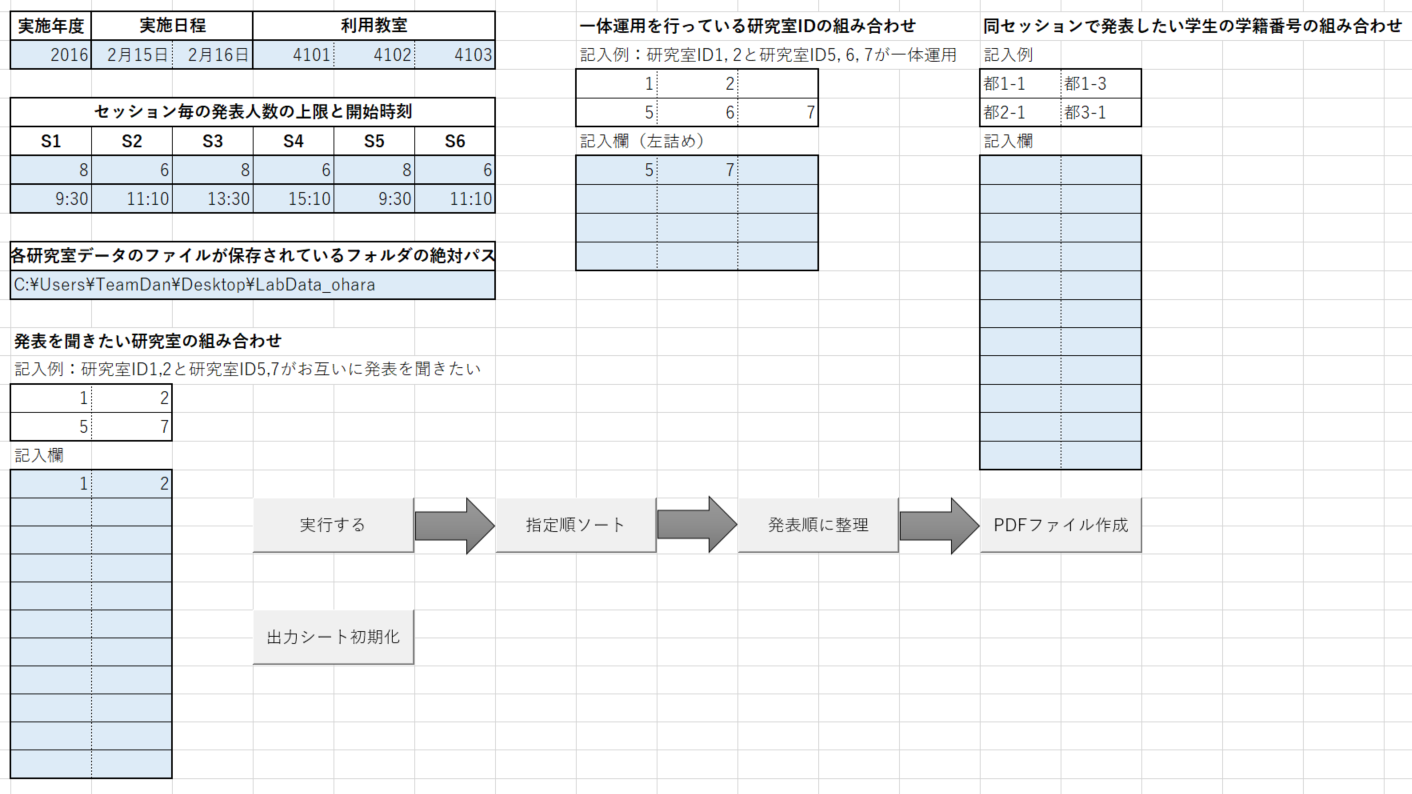
\includegraphics[scale=0.55]{inter.png}
    \caption{入力シート}
    \label{fig:inter}
  \end{center}
\end{figure}

\begin{figure}[H]
  \begin{center}
    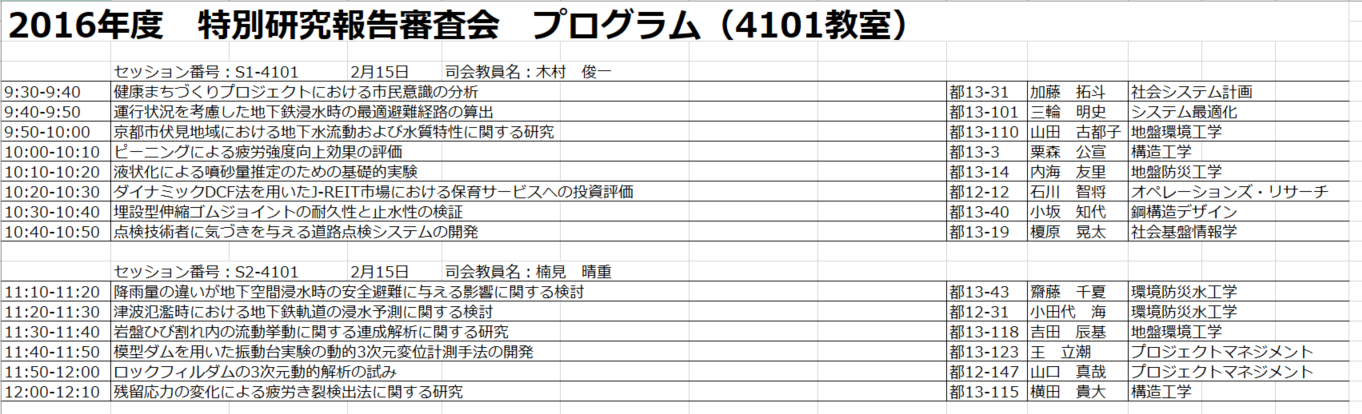
\includegraphics[scale=0.57]{time.png}
    \caption{タイムテーブル 出力例}
    \label{fig:time}
  \end{center}
\end{figure}

\begin{figure}[H]
  \begin{center}
    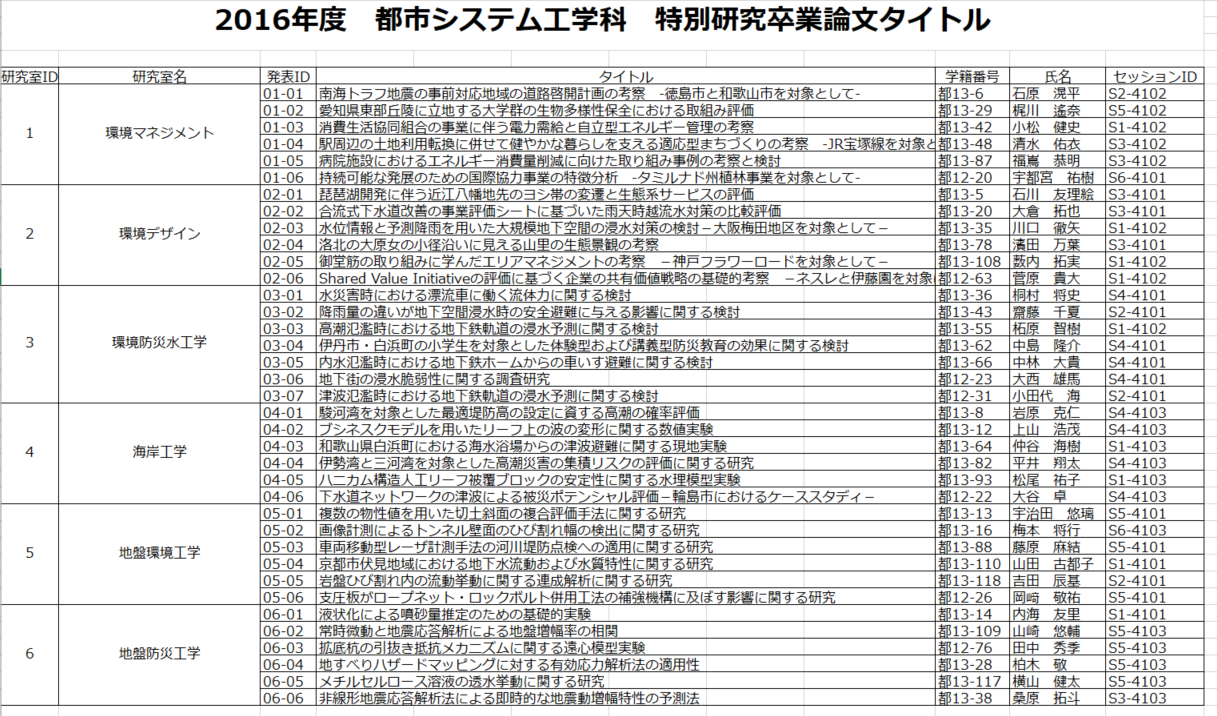
\includegraphics[scale=0.65]{title.png}
    \caption{卒業論文タイトル一覧 出力例}
    \label{fig:title}
  \end{center}
\end{figure}

%%%%%%%%%%%%%%%%%%%%%%%%%%%%%%%%%%%%%%%%%%%%%%%%%%%%%%%%%%%%%%%%%%%%%
\newpage
 \section{数値実験}\label{sec:jikken}
 本章では,本研究で考察対象としている関西大学 環境都市工学部 都市システム工学科の実データを用いて行った数値実験について説明する.
\subsection{計算環境}
本実験で用いた計算環境と最適化ソルバを以下の表\ref{tb:1}に示す.
\begin{table}[H]
  \begin{center}
    \caption{計算環境}\label{tb:1}
    \begin{tabular}{cc} \toprule
      OS & Microsoft Windows 10 Pro \\
      CPU & Intel(R) Core(TM) i7-5600U CPU @ 2.60GHz 2.59GHz\\
      メモリ & 8.00GB \\
      使用ソルバ1 & GLPK $4.47$ \\
      使用ソルバ2 & IBM ILOG CPLEX $12.6.1.0$ \\ \bottomrule
    \end{tabular}
  \end{center}
\end{table}

\subsection{データ概要}
本章で行う数値実験は,関西大学 環境都市工学部 都市システム工学科の $2016$ 年度の研究室・学生数を元に,本実験のために一部改変したデータを用いている.データの概要は以下の通りである.
\begin{itemize}
\item 研究室数 : $21$
\item 学生数 : $124$ 人
\item 各研究室の学生数および担当教員が参加可能な時間帯 : 表 \ref{tb:LabData2016} の通り
 \begin{table}[H]
    \begin{center}
      \caption{各研究室の学生数と担当教員が参加可能な時間帯}
      \label{tb:LabData2016}
      \begin{tabular}{lrrrr} \toprule
        研究室 & 学生数 & $1$ 日目AM & $1$ 日目PM & $2$ 日目AM\\ \toprule
        環境マネジメント & 6 & ○ & ○ & ○\\ \hline
        環境デザイン & 6 & ○ & ○ & ○\\ \hline
        環境防災水工学 & 7 & ○ & ○ & △\\ \hline
        海岸工学 & 6 & ○ & ○ & ○\\ \hline
        地盤環境工学 & 6 & ○ & ○ & ○\\ \hline
        地盤防災工学 & 6 & ○ & ○ & ○\\ \hline
        構造工学 & 6 & ○ & ○ & ○\\ \hline
        鋼構造デザイン & 5 & ○ & ○ & ○\\ \hline
        コンクリート工学 & 6 & ○ & ○ & ○\\ \hline
        複合材料構造 & 5 & ○ & ○ & ○\\ \hline
        プロジェクトマネジメント & 6 & ○ & ○ & ○\\ \hline
        社会資本計画 & 6 & △ & ○ & ○\\ \hline
        都市地域計画 & 5 & ○ & ○ & ○\\ \hline
        交通システム & 5 & ○ & ○ & ○\\ \hline
        オペレーションズ・リサーチ & 6 & ○ & ○ & ○\\ \hline
        社会システム計画 & 5 & ○ & ○ & ○\\ \hline
        ネットワーク工学 & 9 & ○ & ○ & ○\\ \hline
        メディア工学 & 6 & ○ & ○ & ○\\ \hline
        社会基盤情報学 & 7 & ○ & ○ & ○\\ \hline
        システムモデリング & 4 & ○ & ○ & ○\\ \hline
        システム最適化 & 6  & ○ & ○ & △\\ \bottomrule
      \end{tabular}
    \end{center}
    \hspace{1cm} ○:その時間帯に参加可能 \\
    \hspace{1cm} △:その時間帯の一部に参加可能
  \end{table}
\item 一体運用する研究室の組合せ
\begin{itemize}
\item 環境マネジメント研究室と環境デザイン研究室
\end{itemize}
\item 同じセッションで発表するのが望ましい学生の組合せ
\begin{itemize}
\item メディア工学研究室の$2$名
\item 鋼構造デザイン研究室の$2$名
\end{itemize}
\item 関心度が高く発表セッションが重複しないことが望ましい研究室の組合せ
\begin{itemize}
\item 地盤環境工学研究室と地盤防災工学研究室
\item ネットワーク工学研究室とメディア工学研究室
\end{itemize}
\end{itemize}

\subsection{実験 $1$}\label{sec:jikken1}
実験 $1$ では,\ref{sec:tuika}節で説明した$2$種類の制約条件を追加した$2$つのモデルで,制約条件を満たしたスケジュールが作成可能かについての実験と,各セッションで発表できる人数の上限を変更する事による求解時間・目的関数の変化についての実験を行った.求解時間は $10800$ 秒($3$時間)を上限とし,計算時間が $10800$ 秒を超えると,その時点で計算を終了し暫定解を出力した.実験結果を表 \ref{tb:jikkenx1},\ref{tb:jikkeny1} に記す.
\begin{table}[H]
  \begin{center}
    \caption{考慮制約 $5\mathchar`-1$を追加したモデル$1$での実験結果}
    \label{tb:jikkenx1}
    \begin{tabular}{r|ccccccccc}  \toprule
    実験ケース &  S1 & S2 & S3 & S4 & S5 & S6 & 求解時間 (秒) & 目的関数 & gap (\%) \\ \toprule 
    ケース$1$ &  8 & 6 & 8 & 6 & 8 & 6 & 188 & 46 & 0 \\ \hline
    ケース$2$ & 8 & 7 & 8 & 7 & 8 & 7 & 10800 & 46 & 2.17 \\ \hline
    ケース$3$ & 7 & 7 & 7 & 7 & 7 & 7 & 10800 & 47& 2.13 \\ \bottomrule
      \end{tabular}
  \end{center}
  S1, ..., S6:セッション $1$, ..., セッション $6$ で発表できる人数の上限 (人)
\end{table}

\begin{table}[H]
  \begin{center}
    \caption{考慮制約 $5\mathchar`-2$を追加したモデル$2$での実験結果}
    \label{tb:jikkeny1}
    \begin{tabular}{r|ccccccccc} \toprule
     実験ケース & S1 & S2 & S3 & S4 & S5 & S6 & 求解時間 (秒) & 目的関数 & gap (\%) \\ \toprule
     ケース$1$ & 8 & 6 & 8 & 6 & 8 & 6 & 891 & 46 & 0 \\ \hline
     ケース$2$ & 8 & 7 & 8 & 7 & 8 & 7 & 10800 & 46 & 2.17 \\ \hline
     ケース$3$ & 7 & 7 & 7 & 7 & 7 & 7 & 10800 & 48  & 5.12 \\ \bottomrule
      \end{tabular}
  \end{center}
  S1, ..., S6:セッション $1$, ..., セッション $6$ で発表できる人数の上限 (人)
\end{table}
 表\ref{tb:jikkenx1},\ref{tb:jikkeny1} を見ると,どちらのモデルでもスケジュールが作成可能であることが確認できた.また,各セッションで発表できる人数の上限を変更しても目的関数には大きな変化は見られなかった.しかし,各セッションで発表できる人数の上限に,奇数($7$ 人)が増えると,どのケースも求解時間が大幅に伸びることが確認できた.これは昨年度の研究\cite{wakabayasi}でも同様の傾向があると報告されている.つまり,このインターフェースを使用する際は,各セッションの発表人数の上限をなるべく偶数に設定すると短い時間でスケジュールを作成することができるようである.

\subsection{実験 $2$}
実験$2$では,$5$つの考慮制約に重み付けを行い,目的関数がどのように変化するのかを確認する実験を行った.この実験では,考慮制約 $5\mathchar`-2$を追加したモデル$2$を使用した.また本実験では,各セッションの人数の上限を表\ref{tb:jk}の$3$ケースに設定した.
\begin{table}[H]
  \begin{center}
    \caption{実験ケース}
    \label{tb:jk}
    \begin{tabular}{r|cccccc} \toprule
     実験ケース & $S1$ & $S2$ & $S3$ & $S4$ & $S5$ & $S6$\\ \toprule
     ケース$1$ & 8 & 6 & 8 & 6 & 8 & 6\\
     ケース$2$ & 8 & 7 & 8 & 7 & 8 & 7 \\ 
     ケース$3$ & 7 & 7 & 7 & 7 & 7 & 7 \\ \bottomrule
      \end{tabular}
  \end{center}
 \hspace{2cm} $ S1$, ..., $S5$:セッション $1$, ..., セッション $5$ で発表できる人数の上限(人)
\end{table}

\subsubsection{実験$2\mathchar`-1$}
まず,考慮制約の重み$w_i(i=1,...,5)$をすべて$1$にした状態で,$5$つの考慮制約の違反量がそれぞれどのような値になるかを確認した.実験結果を表\ref{tb:jikkeny2}にまとめた.
\begin{table}[H]
  \begin{center}
    \caption{各考慮制約の違反量}
    \label{tb:jikkeny2}
    \begin{tabular}{r|ccccc} \toprule
     実験ケース & $p_1$ & $p_2$ & $p_3$ & $p_4$ & $p_5$ \\ \toprule
     ケース$1$ & 1 & 1 & 44 & 0 & 0 \\
     ケース$2$ & 1 & 1 & 44 & 0 & 0 \\ 
     ケース$3$ & 1 & 3 & 44 & 0 & 0 \\ \bottomrule
      \end{tabular}
  \end{center}
 \hspace{3cm} $ p_1$, ..., $p_5$:考慮制約 $1$, ..., 考慮制約 $5$ での違反量の合計
\end{table}
表\ref{tb:jikkeny2}を見ると,どのケースも考慮制約$3$の違反量の合計値$p_3$がとても大きいことが確認できた.そこで,$3$つの実験ケースにおいて考慮制約$3$の重みを変え,目的関数の値がどのように変化するのかを確認した.実験結果を表\ref{tb:hyou8}にまとめた.
\begin{table}[H]
  \begin{center}
    \caption{重み付けによる目的関数と違反量の変化}
    \label{tb:hyou8}
    \begin{tabular}{r|ccccccc} \toprule
     実験ケース & $p_3$の重み & 目的関数 & $p_1$ & $p_2$ & $p_3$ & $p_4$ & $p_5$ \\ \toprule
      & 1 & 46 & 1 & 1 & 44 & 0 & 0 \\ \cline{2-8}
    ケース$1$ & 2 & 90 & 1 & 1 & 88 & 0 & 0 \\ \cline{2-8}
      & 5 & 222 & 1 & 1 & 220 & 0 & 0 \\ \hline
        & 1 & 46 & 1 & 1 & 44 & 0 & 0 \\ \cline{2-8}
    ケース$2$ & 2 & 90 & 1 & 1 & 88 & 0 & 0 \\ \cline{2-8}
      & 5 & 222 & 1 & 1 & 220 & 0 & 0 \\ \hline
        & 1 & 48 & 1 & 3 & 44 & 0 & 0 \\ \cline{2-8}  
    ケース$3$ & 2 & 91 & 1 & 2 & 88 & 0 & 0 \\ \cline{2-8}
      & 5 & 223 & 1 & 2 & 220 & 0 & 0 \\ \toprule
      \end{tabular}
  \end{center}
  \hspace{2cm} $p_1$, ..., $p_5$:考慮制約 $1$, ..., 考慮制約 $5$ での違反量の合計
\end{table}
表\ref{tb:hyou8}を見ると,考慮制約$3$の重みを他の考慮制約に対して相対的に大きくしたにも関わらず,$p_3$を重みで割った値は一定$(=44)$である.この結果から,今回の実験で発生する$p_3$の値は$44$が最小である可能性があることが分かった.このことを確認するために,次の実験$2\mathchar`-2$を行った.

\subsubsection{実験$2\mathchar`-2$}
この実験では,考慮制約$3$の違反量$p_3$の値が$43$以下になるという絶対制約を加え,スケジュールが作成可能かどうかを確認した.実験結果を\ref{tb:jikkenyz}にまとめた.
\begin{table}[H]\
  \begin{center}
    \caption{実験$2\mathchar`-2$の結果}
    \label{tb:jikkenyz}
    \begin{tabular}{r|c} \toprule
    実験ケース & 実験結果\\ \toprule
    ケース$1$ & 実行可能解なし\\
    ケース$2$ & 実行可能解なし\\
    ケース$3$ & 実行可能解なし\\ \toprule
    \end{tabular}
    \end{center}
\end{table}
表\ref{tb:jikkenyz}を見ると,どのケースも実行可能解がないという結果が得られた.この結果から,今回の実験で使用したデータでは,考慮制約$3$の違反量は$44$が最小であることが確認できた.

\subsection{実験$3$}
この実験では,考慮制約$4$と考慮制約$5$のどちらかが必ず違反するような状態を意図的に作り,重み付けを行うことで目的関数に変化が出るかどうかを確認した.
この実験では,実験$1$,$2$で使用したデータを一部変更したデータを使用して実験を行った.変更した部分は以下の通りである.
\begin{itemize}
\item 一体運用する研究室の組合せ
\begin{itemize}
\item 海岸工学研究室とオペレーションズ・リサーチ研究室
\end{itemize}
\item 同じセッションで発表することが望ましい学生の組合せ
\begin{itemize}
\item 海岸工学研究室とオペレーションズ・リサーチ研究室の学生
\end{itemize}
\end{itemize}
また,本実験における各セッションの人数の上限は,表\ref{tb:jk}のケース$1$とした.
実験結果を表\ref{tb:jikkeny3}にまとめた.
\begin{table}[H]
  \begin{center}
    \caption{重み付けによる目的関数の変化}
    \label{tb:jikkeny3}
    \begin{tabular}{c|cccccc} \toprule
  重みの有無 & 目的関数 & $p_1$ & $p_2$ & $p_3$ & $p_4$ & $p_5$ \\ \toprule
  重みなし & $47$ & $1$ & $1$ & $44$ & $0$ & $1$ \\
  $p_5$に重み付け & $49$ & $1$ & $1$ & $44$ & $3$ & $0$\\ \toprule
    \end{tabular}
    \end{center}
    \hspace{2cm} $p_1$, ..., $p_5$:考慮制約 $1$, ..., 考慮制約 $5$ での違反量の合計
\end{table}

表\ref{tb:jikkeny3}を見ると,重み付けを行っていない状態では,考慮制約$5$の違反量$p_5$の値が$1$になっていた.しかし,$p_5$に重み付けを行うと$p_5$の値は$0$になり,その代わりに考慮制約$4$の違反量$p_4$の値が増えている.この結果から,考慮制約に重み付けを行うことで,考慮制約の重要度を調整することが可能であることを確認できた.

%%%%%%%%%%%%%%%%%%%%%%%%%%%%%%%%%%%%%%%%%%%%%%%%%%%%%%%%%%%%%%%%%%%%%%
\newpage
\section{$2017$ 年度の特別研究報告審査会のスケジュール作成}
本章では,実際に作成した$2017$年度の特別研究報告審査会のスケジュールについて説明する.

本研究では,考慮制約 $5\mathchar`-1$ を追加したモデル$1$と,考慮制約 $5\mathchar`-2$ を追加したモデル$2$を作成し,\ref{sec:jikken}章で数値実験を行った.その結果それぞれのモデルでスケジュールが作成可能であることを確認した.しかし,モデル$1$は,関心度が高く発表を聞きに行きたい研究室の組合せが増えると,同一セッション内で複数回教室を移動しなければならない可能性があった.一方,モデル$2$ は,同一セッション内で教室を移動する必要はなく,移動回数が少ない.そこで,本研究では作成した$2$つのモデルの内,モデル$2$を使用しスケジュールを作成した.

\subsection{データ概要}\label{sec:data}
使用したデータの概要は以下の通りである.
\begin{itemize}
\item 研究室数 : $20$
\item 学生数 : $128$ 人
\item 各研究室の学生数および担当教員が参加可能な時間帯 : 表 \ref{tb:LabData2017} の通り
 \begin{table}[H]
    \begin{center}
      \caption{各研究室の学生数と担当教員が参加可能な時間帯}
      \label{tb:LabData2017}
      \begin{tabular}{lrrrr} \toprule
        研究室 & 学生数 & $1$ 日目AM & $1$ 日目PM & $2$ 日目AM\\ \toprule
        環境マネジメント & 8 & ○ & ○ & ○\\ \hline
        環境防災水工学 & 6 & ○ & ○ & ○\\ \hline
        海岸工学 & 7 & ○ & ○ & ○\\ \hline
        地盤環境工学 & 6 & ○ & ○ & ○\\ \hline
        地盤防災工学 & 6 & ○ & ○ & △\\ \hline
        構造工学 & 6 & ○ & ○ & ○\\ \hline
        鋼構造デザイン & 5 & ○ & ○ & ○\\ \hline
        コンクリート工学 & 6 & ○ & ○ & ○\\ \hline
        複合材料構造 & 6 & ○ & ○ & ○\\ \hline
        プロジェクトマネジメント & 6 & ○ & ○ & ○\\ \hline
        社会資本計画 & 7 & ○ & ○ & ○\\ \hline
        都市地域計画 & 6 & ○ & ○ & ○\\ \hline
        交通システム & 6 & ○ & ○ & ○\\ \hline
        オペレーションズ・リサーチ & 6 & ○ & ○ & ○\\ \hline
        社会システム計画 & 7 & ○ & ○ & $\times$\\ \hline
        ネットワーク工学 & 8 & ○ & △ & ○\\ \hline
        メディア工学 & 7 & ○ & ○ & ○\\ \hline
        社会基盤情報学 & 6 & ○ & ○ & ○\\ \hline
        システムモデリング & 6 & ○ & ○ & △\\ \hline
        システム最適化 & 7  & ○ & ○ & ○\\ \bottomrule
      \end{tabular}
    \end{center}
    \hspace{1cm} ○:その時間帯に参加可能 \\
    \hspace{1cm} △:その時間帯の一部に参加可能\\
    \hspace{0.94cm} \ $\times$:その時間帯に参加不可能
  \end{table}
\item 一体運用する研究室の組合せ
\begin{itemize}
\item 都市地域計画研究室と交通システム研究室
\end{itemize}
\item 同じセッションで発表するのが望ましい学生の組合せ
\begin{itemize}
\item 社会システム研究室の$2$名
\end{itemize}
\item 関心度が高く発表セッションが重複しないことが望ましい研究室の組合せ
\begin{itemize}
\item 海岸工学研究室と環境防災水工学研究室
\item コンクリート工学研究室と複合材料構造研究室
\item 複合材料構造研究室と構造工学研究室
\item 複合材料構造研究室と鋼構造デザイン研究室
\item オペレーションズ・リサーチ研究室と社会システム研究室
\item オペレーションズ・リサーチ研究室とシステム最適化研究室
\end{itemize}
\end{itemize}

\subsection{作成したスケジュール}
\ref{sec:data}節のデータを元に$2017$年度のスケジュールを作成した.図\ref{fig:timeo},図\ref{fig:titleo}は実際に作成したスケジュールのタイムテーブルと,タイトル一覧表の一部である.
\begin{figure}[H]
  \begin{center}
    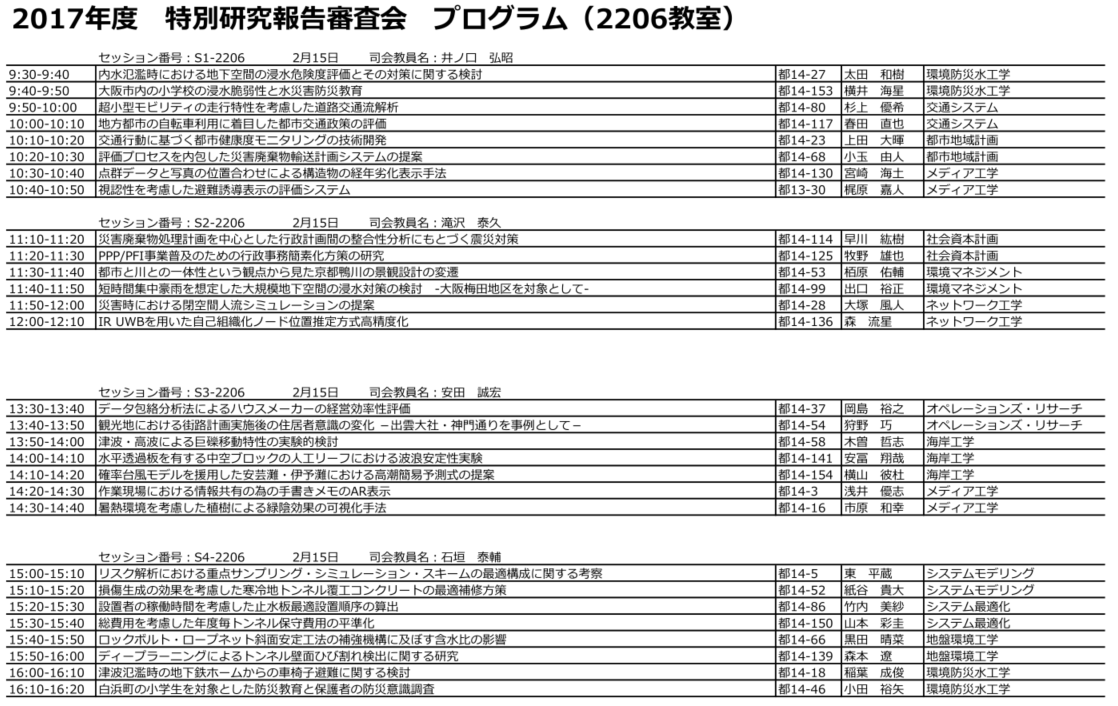
\includegraphics[scale=0.7]{tiomeo.png}
    \caption{タイムテーブル}
    \label{fig:timeo}
  \end{center}
\end{figure}

\begin{figure}[H]
  \begin{center}
    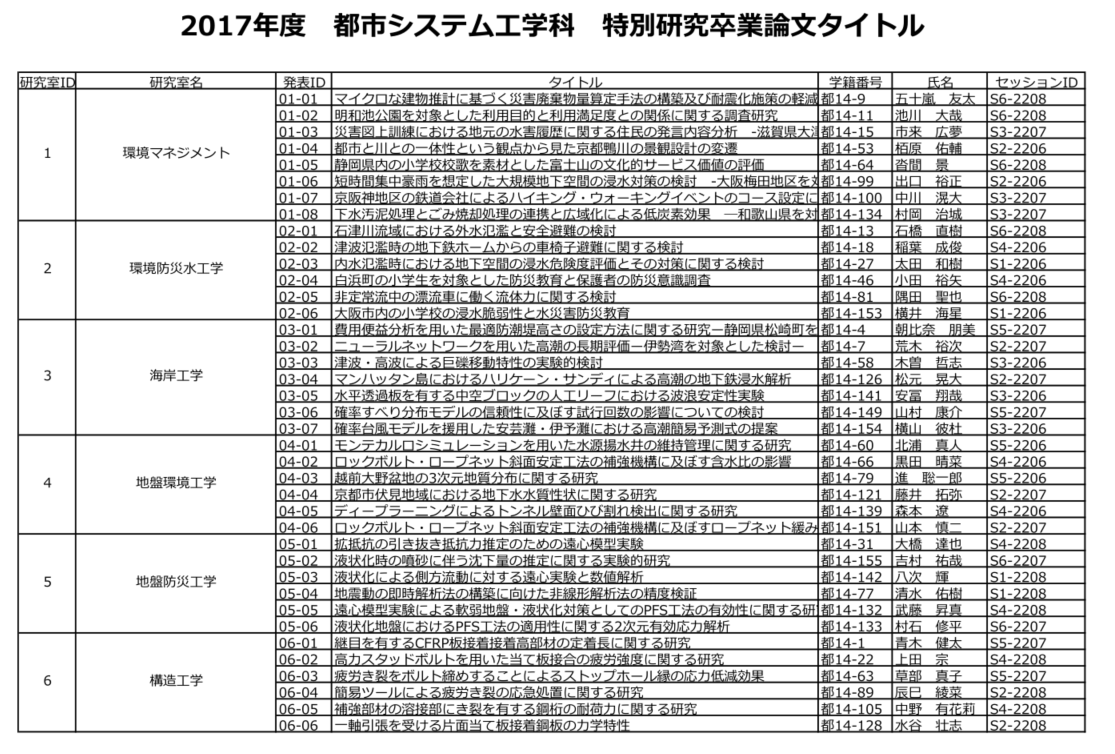
\includegraphics[scale=0.7]{titleo.png}
    \caption{タイトル一覧表}
    \label{fig:titleo}
  \end{center}
\end{figure}

このスケジュールを作成した際の目的関数と各考慮制約の違反量を表\ref{tb:2017}にまとめる.
\begin{table}[H]
  \begin{center}
    \caption{目的関数と違反量}
    \label{tb:2017}
    \begin{tabular}{cccccc} \toprule
    目的関数 & $p_1$ & $p_2$ & $p_3$ & $p_4$ & $p_5$ \\ \hline
    $47$ & $1$ & $2$ & $44$ & $0$ & $0$\\ \toprule
    \end{tabular}
    \end{center}
    \hspace{3cm} $p_1$, ..., $p_5$:考慮制約 $1$, ..., 考慮制約 $5$ での違反量の合計
\end{table}
表\ref{tb:2017}を見ると,$p_4$と$p_5$の値が$0$になっている.つまり,今年度のスケジュールでは,考慮制約$4$と考慮制約$5$はすべて満たせているということである.実際にスケジュールを確認すると,同じセッションで発表することが望ましいとされていた社会システム研究室の$2$名は,同じセッションで発表を行っている.また,関心度が高く発表を聞きに行きたい研究室同士の発表セッションはすべて重複しておらず,発表を聞きに行くことが可能なスケジュールになっている.

\subsection{作成したスケジュールの問題点}
本研究で作成した $2017$年度のスケジュールには問題点があった.問題点は,ある研究室が$4$つのセッションで発表を行うようなスケジュールになっていたという点である.作成したスケジュールを確認すると,図\ref{fig:kubota}のように,社会基盤情報学研究室が$4$つのセッションで発表するようなスケジュールになっていた.

\begin{figure}[H]
  \begin{center}
    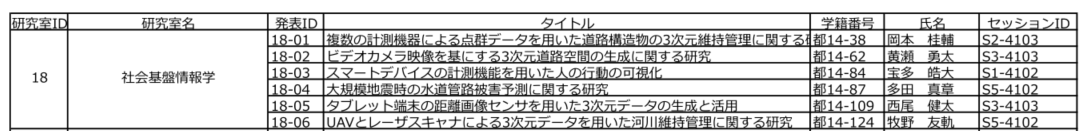
\includegraphics[scale=0.75]{kubota.png}
    \caption{社会基盤情報学の情報}
    \label{fig:kubota}
  \end{center}
\end{figure}

しかし$1$つの研究室が$4$つのセッションで発表することは,その研究室の担当教員への負担が大きいため避けたい.そのため,今年度のスケジュールでは,手動で社会基盤情報学研究室の学生の発表セッションを移動させ,図\ref{fig:kubotaa}のように$3$つのセッションで発表を行うようなスケジュールに修正した.

\begin{figure}[H]
  \begin{center}
    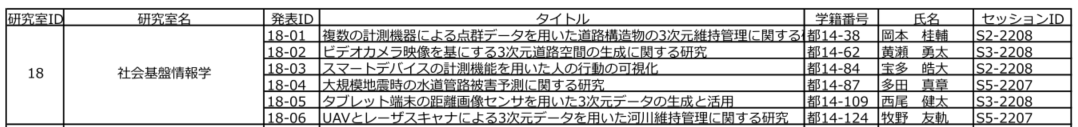
\includegraphics[scale=0.75]{kubotaa.png}
    \caption{修正後の社会基盤情報学の情報}
    \label{fig:kubotaa}
  \end{center}
\end{figure}

今回このような問題が発生した原因として,絶対制約 $3 $の定式化に間違いがあったことが考えられる.絶対制約 $3$ は以下のような内容であった.

\begin{description}
\item[絶対制約 $3$] 各研究室は複数のセッションで発表する.
\begin{eqnarray}\label{eq:c3}
    \sum_{s \in S, r \in R} y_{s,r,l} \geq 2 \quad (l \in L)
  \end{eqnarray}
\end{description}

この制約条件は,各研究室が必ず$2$つ以上のセッションで発表するという内容になっていた.しかし実際は,各研究室は$3$つのセッションで発表することが望ましい.そのため,(\ref{eq:c3})は本質的には間違いであった.

昨年度のスケジュールでは,各研究室が$3$つのセッションで発表するように偶然なっていた.しかし,今年度のスケジュールでは,$4$つのセッションで発表する研究室が存在するスケジュールになってしまった.これを回避するために絶対制約$3$を以下の(\ref{eq:c3k})のようにする必要があることが分かった.

\begin{description}
\item[絶対制約 $3$] 各研究室は$3$つのセッションで発表する.
\begin{eqnarray}\label{eq:c3k}
    \sum_{s \in S, r \in R} y_{s,r,l} = 3 \quad (l \in L)
  \end{eqnarray}
\end{description}

以上が本研究で作成したスケジュールの問題点である.


%%%%%%%%%%%%%%%%%%%%%%%%%%%%%%%%%%%%%%%%%%%%%%%%%%%%%%%%%%%%%%%%%%%%%%
\newpage
\section{おわりに}
本研究では,昨年度の研究\cite{wakabayasi}で挙げられた検討すべき事項の改良と,頂いた要望を実現するために新たな制約条件を追加した最適化モデルを作成した.具体的には,関心度が高く発表を聞きに行きたい研究室があった場合,その研究室の発表をできるだけ聞きに行けるようにするという制約条件を追加しスケジュールを作成した.その結果,要望を満たしたスケジュールを作成することができた.しかし,一部,望ましくないと思われる個所を手作業で修正した.

今後の課題として,より万人にとって「最適なスケジュール」となるように制約条件の追加・変更を行う必要があると考える.「最適なスケジュール」とは,人により解釈が異なるものである.そのため,今後調査を行い,より万人にとって「最適なスケジュール」となるように最適化モデルを改良する必要がある.

%%%%%%%%%%%%%%%%%%%%%%%%%%%%%%%%%%%%%%%%%%%%%%%%%%%%%%%%%%%%%%%%%%%%%%
\newpage
\section*{謝辞}
本研究を進めるにあたり,ご指導いただいた檀寛成准教授に深く感謝致します.また,日ごろの議論を通じて多くの知識や示唆をいただいたシステム最適化研究室の皆様に心から感謝の気持ちと御礼を申し上げたく謝辞にかえさせていただきます.

\begin{flushright} 
平成 $30$ 年 $2$ 月 $10$ 日
\end{flushright} 

%%%%%%%%%%%%%%%%%%%%%%%%%%%%%%%%%%%%%%%%%%%%%%%%%%%%%%%%%%%%%%%%%%%%%%
% 参考文献
% 本文で参照する際は\citeを使用
\newpage
\begin{thebibliography}{99}
\bibitem{VBA2}大村 あつし,日常業務の自動化からアプリケーション開発まで ExcelVBA 本格入門,技術評論社,$12$-$15$ ($2015$).
\bibitem{VBA3}唐松 隆志,仕事を早くする ExcwlVBA 入門,日経BP社,$6$-$8$ ($2015$)
\bibitem{VBA1}門脇 香奈子,今すぐ使えるかんたん Ex Excel&マクロ VBA プロ技セレクション,技術評論社,$20$-$24$ ($2015$).
\bibitem{CSP}清水 良明,最適工学のすすめ 賢い決め方のワークベンチ,コロナ社,$159$ ($2010$).
\bibitem{Math}田村 明久,村松 正和,最適化法,共立出版株式会社,$1$-$3$ ($2002$).
\bibitem{wakabayasi}若林 裕麻,特別研究報告審査会のスケジュール作成の自動化,関西大学環境都市工学部 卒業論文 ($2017$).
\bibitem{GLPK}GLPK - GNU Project - Free Software Foundation (FSF), \par \verb|https://www.gnu.org/software/glpk/|($2018$年 $1$ 月 $25$ 日確認).
\bibitem{CPLEX}IBM CPLEX Optimizer - United States, \par \verb|http://www-01.ibm.com/software/commerce/optimization/cplex-optimizer/| \par($2018$ 年 $1$ 月 $25$ 日確認).
\end{thebibliography}

%%%%%%%%%%%%%%%%%%%%%%%%%%%%%%%%%%%%%%%%%%%%%%%%%%%%%%%%%%%%%%%%%%%%%%
 \newpage
 \appendix
% 付録になると章番号がアルファベットに変わります.
%%%%%%%%%%%%%%%%%%%%%%%%%%%%%%付録%%%%%%%%%%%%%%%%%%%%%%%%%%%%%%%%%%%%
\section{本研究で使用した最適化問題のモデルファイル・データファイル}
\subsection{モデルファイル}
\subsubsection{モデル$1$}
\begin{verbatim}
set D;             #//時間帯
set S;             #//セッション
set S_{D};         #//セッションの組み合わせ
set R;             #//教室
set A{S};          #//セッション S での発表順序
set I;             #//生徒の学籍番号
set L;             #//研究室 
set O dimen 2;     #//一体運用している研究室の組み合わせ
set C dimen 2;     #//同セッションで発表したい学生の学籍番号の組み合わせ
set G dimen 2;     #//発表を聞きたい研究室の組み合わせ

param u{S};                              #//セッション毎の発表人数の上限
param b{L,I} binary default 0;           #//学生が所属する研究室
param j{S, I} binary default 1;          #//学生が参加可能なセッション
param j_{S, L} binary default 1;         #//教員が参加可能なセッション

var x{s in S, R, I, A[s]} binary;        #//発表するかどうか(個人単位)
var y{S, R, L} binary;                   #//発表するかどうか(研究室単位)
var n_s{S, R},integer;                   #//各セッションの発表人数
var n_d{D, L},integer;                   #//各研究室の日程毎の発表人
var c{S, R, L} binary;                   #//教員が司会をするかどうか
var p1{S} binary;                        #//違反の有無(考慮制約1について)
var p2{D, L} binary;                     #//違反の有無(考慮制約2について)
var p3{D, D, L},integer;                 #//違反量  (考慮制約3について)
var p4{C} binary;                        #//違反の有無(考慮制約4について)
var p5{G} binary;                        #//違反の有無(考慮制約5について)


minimize Objective:
sum {s in S} p1[s] + sum {d in D, l in L} p2[d,l] + sum {d1 in D, d2 in D, l in L : d1 != d2 } p3[d1,d2,l]
 + sum{(i1, i2) in C} p4[i1,i2] + sum{(l_1,l_2) in G} p5[l_1,l_2]; 


#//全学生が1回発表する
subject to AllStudentOnePublish {i in I}:
 sum {s in S, r in R, a in A[s]} x[s,r,i,a] == 1;

#//学生は教員・自身が共に参加可能なセッションで発表できる
subject to AvailableSession
 {s in S, r in R, l in L, i in I, a in A[s] : b[l,i] == 1}:
 x[s,r,i,a] <= j[s,i] * j_[s,l];

#//各研究室は最低2セッションで発表する
subject to OneLabOverTwoRoom {l in L}:
 sum {s in S, r in R} y[s,r,l] >= 2;

#//同時刻のセッションで教室をまたいで発表しない
subject to OneTimeOneSession {s in S, l in L}:
 sum {r in R} y[s,r,l] <= 1;

#//研究室での発表がある場合,(その研究室の)学生が発表できる
subject to RelationPersonalAndLab1
 {s in S, r in R, l in L, i in I : b[l,i] == 1}:
 sum {a in A[s]} x[s,r,i,a] <= y[s,r,l];

#//研究室の発表がある場合,(その研究室の)誰かしらは発表する
subject to RelationPersonalAndLab2 {s in S, r in R, l in L}:
 y[s,r,l] <= sum {i in I, a in A[s] : b[l,i]==1} x[s,r,i,a];

#//一体運用を行う研究室は同セッションにて発表する
subject to OneOperation {s in S, r in R, (l1, l2) in O}:
 y[s,r,l1] == y[s,r,l2];

#//各セッションの発表人数の計算
subject to NumOfSession {s in S, r in R}:
 n_s[s,r] == sum {i in I, a in A[s]} x[s,r,i,a];

#//各セッションの発表者数は上限を超えない
subject to UpperBoundOfSession {s in S, r in R}:
 n_s[s,r] <= u[s];

#//各研究室の,日程毎の発表者数
subject to NumOfPublishers {d in D, l in L}:
 n_d[d,l] == sum {s_ in S_[d], r in R, i in I, a in A[s_] :b[l,i] == 1}
 x[s_,r,i,a];

#//全セッションで教員の誰かが司会をする
subject to AllSessionHaveChairman {s in S, r in R}:
 sum {l in L} c[s,r,l] == 1;

#//研究室での発表がある場合,(その研究室の)教員が司会をすることがある
subject to ConditionOfChairman {s in S, r in R, l in L}:
 c[s,r,l] <= y[s,r,l];

#//各教員が司会をするのは1度まで
subject to OneLabOneChairman {l in L}:
 sum {s in S, r in R} c[s,r,l] <= 1;

#//同一セッション・教室内での発表順序が重ならない
subject to DifferenceOrder {s in S, r in R, a in A[s]}:
 sum {i in I} x[s,r,i,a] <= 1;

	
#//同時刻のセッションにおいて,発表人数の最大と最小の差は1以下
subject to DifferenceNumOfPublishers {s in S, r1 in R, r2 in R : r1 != r2}:
 n_s[s,r1] - n_s[s,r2] <= p1[s];

#//各研究室は1日目AM,1日目PM,2日目AMのそれぞれで発表するのが望ましい
subject to AllDaysPublish_L {d in D, l in L}:
 - p2[d,l] <= sum {r in R, s in S_[d]} (y[s,r,l])- 1;

subject to AllDaysPublish_R {d in D, l in L}:
 sum {r in R, s in S_[d]} (y[s,r,l]) - 1 <= p2[d,l];

#//各研究室の中で,日程毎の発表者数の差は,少ない状態が望ましい
subject to DifferenceBetweenDays_L {d1 in D, d2 in D, l in L : d1 != d2 }:
 -p3[d1,d2,l] <= n_d[d1,l] - n_d[d2,l];

subject to DifferenceBetweenDays_R {d1 in D, d2 in D, l in L : d1 != d2}:
 n_d[d1,l] - n_d[d2,l] <= p3[d1,d2,l];

#//個人単位で同セッションで発表したい組み合わせをできるだけ成立させる
subject to IdCombination_L {s in S, r in R, (i1, i2) in C}:
 sum{a in A[s]} x[s,r,i1,a] - sum{a in A[s]} x[s,r,i2,a] <= p4[i1,i2];

subject to IdCombination_R {s in S, r in R, (i1, i2) in C}:
 -p4[i1,i2] <=sum {a in A[s]} x[s,r,i1,a] - sum{a in A[s]} x[s,r,i2,a];

#//発表を聞きたい研究室の学生の発表スロットができるだけ重ならない
subject to MakeGallery_x
 {s in S, a in A[s], i_1 in I, i_2 in I, (l_1, l_2) in G : b[l_1,i_1] == 1 && b[l_2,i_2] == 1}:
 sum {r in R} (x[s,r,i_1,a] + x[s,r,i_2,a]) - 1 <= p5[l_1,l_2];
\end{verbatim}
\subsubsection{モデル$2$}
\begin{verbatim}
set D;             #//時間帯
set S;             #//セッション
set S_{D};         #//セッションの組み合わせ
set R;             #//教室
set A{S};          #//セッション S, 教室 R での発表順序
set I;             #//生徒の学籍番号
set L;             #//研究室 
set O dimen 2;     #//一体運用している研究室の組み合わせ 
set C dimen 2;     #//同セッションで発表したい学生の学籍番号の組み合わせ 
set G dimen 2;     #//研究を聞きたい研究室の組み合わせ)


param u{S};                               #//セッション毎の発表人数の上限
param b{L,I} binary default 0;            #//学生が所属する研究室
param j{S, I} binary default 1;           #//学生が参加可能なセッション
param j_{S, L} binary default 1;          #//教員が参加可能なセッション

var x{s in S, R, I, A[s]} binary;         #//発表するかどうか(個人単位)
var y{S, R, L} binary;                    #//発表するかどうか(研究室単位)
var n_s{S, R},integer;                    #//各セッションの発表人数
var n_d{D, L},integer;                    #//各研究室の日程毎の発表人
var c{S, R, L} binary;                    #//教員が司会をするかどうか
var p1{S} binary;                         #//違反の有無(考慮制約1について)
var p2{D, L} binary;                      #//違反の有無(考慮制約2について)
var p3{D, D, L},integer;                  #//違反量  (考慮制約3について)
var p4{C} binary;                         #//違反の有無(考慮制約4について)
var p5{G} binary;                         #//違反の有無(考慮制約5について)


minimize Objective:
 sum {s in S} p1[s] + sum {d in D, l in L} p2[d,l] + sum {d1 in D, d2 in D, l in L : d1 != d2 } p3[d1,d2,l]
 + sum{(i1, i2) in C} p4[i1,i2] + sum{(l1,l2) in G} p5[l1,l2];


#//全学生が1回発表する
subject to AllStudentOnePublish {i in I}:
 sum {s in S, r in R, a in A[s]} x[s,r,i,a] == 1;

#//学生は教員・自身が共に参加可能なセッションで発表できる
subject to AvailableSession
 {s in S, r in R, l in L, i in I, a in A[s] : b[l,i] == 1}:
 x[s,r,i,a] <= j[s,i] * j_[s,l];

#//各研究室は最低2セッションで発表する
subject to OneLabOverTwoRoom {l in L}:
 sum {s in S, r in R} y[s,r,l] >= 2;

#//同時刻のセッションで教室をまたいで発表しない
subject to OneTimeOneSession {s in S, l in L}:
 sum {r in R} y[s,r,l] <= 1;

#//研究室での発表がある場合,(その研究室の)学生が発表できる
subject to RelationPersonalAndLab1
 {s in S, r in R, l in L, i in I : b[l,i] == 1}:
 sum {a in A[s]} x[s,r,i,a] <= y[s,r,l];

#//研究室の発表がある場合,(その研究室の)誰かしらは発表する
subject to RelationPersonalAndLab2 {s in S, r in R, l in L}:
 y[s,r,l] <= sum {i in I, a in A[s] : b[l,i]==1} x[s,r,i,a];

#//一体運用を行う研究室は同セッションにて発表する
subject to OneOperation {s in S, r in R, (l1, l2) in O}:
 y[s,r,l1] == y[s,r,l2];

#//各セッションの発表人数の計算
subject to NumOfSession {s in S, r in R}:
 n_s[s,r] == sum {i in I, a in A[s]} x[s,r,i,a];

#//各セッションの発表者数は上限を超えない
subject to UpperBoundOfSession {s in S, r in R}:
 n_s[s,r] <= u[s];

#//各研究室の,日程毎の発表者数
subject to NumOfPublishers {d in D, l in L}:
 n_d[d,l] == sum {s_ in S_[d], r in R, i in I, a in A[s_] :b[l,i] == 1}
 x[s_,r,i,a];

#//全セッションで教員の誰かが司会をする
subject to AllSessionHaveChairman {s in S, r in R}:
 sum {l in L} c[s,r,l] == 1;

#//研究室での発表がある場合,(その研究室の)教員が司会をすることがある
subject to ConditionOfChairman {s in S, r in R, l in L}:
 c[s,r,l] <= y[s,r,l];

#//各教員が司会をするのは1度まで
subject to OneLabOneChairman {l in L}:
 sum {s in S, r in R} c[s,r,l] <= 1;

#//同一セッション・教室内での発表順序が重ならない
subject to DifferenceOrder {s in S, r in R, a in A[s]}:
 sum {i in I} x[s,r,i,a] <= 1;

	
#//同時刻のセッションにおいて,発表人数の最大と最小の差は1以下
subject to DifferenceNumOfPublishers {s in S, r1 in R, r2 in R : r1 != r2}:
 n_s[s,r1] - n_s[s,r2] <= p1[s];

#//各研究室は1日目AM,1日目PM,2日目AMのそれぞれで発表するのが望ましい
subject to AllDaysPublish_L {d in D, l in L}:
 - p2[d,l] <= sum {r in R, s in S_[d]} (y[s,r,l])- 1;

subject to AllDaysPublish_R {d in D, l in L}:
 sum {r in R, s in S_[d]} (y[s,r,l]) - 1 <= p2[d,l];

#//各研究室の中で,日程毎の発表者数の差は,少ない状態が望ましい
subject to DifferenceBetweenDays_L {d1 in D, d2 in D, l in L : d1 != d2 }:
 -p3[d1,d2,l] <= n_d[d1,l] - n_d[d2,l];

subject to DifferenceBetweenDays_R {d1 in D, d2 in D, l in L : d1 != d2}:
 n_d[d1,l] - n_d[d2,l] <= p3[d1,d2,l];

#//個人単位で同セッションで発表したい組み合わせをできるだけ成立させる
subject to IdCombination_L {s in S, r in R, (i1, i2) in C}:
 -p4[i1,i2] <=sum{a in A[s]} x[s,r,i1,a] -sum{a in A[s]} x[s,r,i2,a];

subject to IdCombination_R {s in S, r in R, (i1, i2) in C}:
 sum{a in A[s]} x[s,r,i1,a] - sum{a in A[s] }x[s,r,i2,a] <= p4[i1,i2];


#//お互いに発表を聞きたい研究室の発表セッションができるだけ重ならない
subject to MakeGallery {s in S, (l1, l2) in G}:
 sum {r in R} ( y[s,r,l1] + y[s,r,l2] ) - 1 <= p5[l1,l2];
\end{verbatim}
\subsection{データファイル}
\subsubsection{数値実験に使用したデータファイル}
\begin{verbatim}
set D := d1AM d1PM d2AM;
set S_[d1AM] := 1 2;
set S_[d1PM] := 3 4;
set S_[d2AM] := 5 6;
set S :=
 1 
 2 
 3 
 4 
 5 
 6 
;
set R :=
 4101 
 4102 
 4103 
;
set O :=
(1,2)
;
set C :=
(13-72,13-113)
(13-58,13-80)
;
set G:=
(5,6)
(17,18)
;
param u :=
1 8
2 6
3 8
4 6
5 8
6 6
;
set L :=
 1 
 2 
 3 
 4 
 5 
 6 
 7 
 8 
 9 
 10 
 11 
 12 
 13 
 14 
 15 
 16 
 17 
 18 
 19 
 20 
 21 
;
set A[1] := 1 2 3 4 5 6 7 8; 
set A[2] := 1 2 3 4 5 6 7 8; 
set A[3] := 1 2 3 4 5 6 7 8; 
set A[4] := 1 2 3 4 5 6 7 8; 
set A[5] := 1 2 3 4 5 6 7 8; 
set A[6] := 1 2 3 4 5 6 7 8; 
set I :=
13-6
13-29
13-42
13-48
13-87
12-20
13-5
13-20
13-35
13-78
13-108
12-63
13-36
13-43
13-55
13-62
13-66
12-23
12-31
13-8
13-12
13-64
13-82
13-93
12-22
13-13
13-16
13-88
13-110
13-118
12-26
13-14
13-109
12-76
13-28
13-117
13-38
13-3
13-54
13-68
13-105
13-115
12-80
13-26
13-40
13-58
13-96
12-110
13-7
13-25
13-70
13-79
13-86
12-52
11-88
13-44
13-69
13-80
13-106
13-46
13-75
13-98
13-123
12-108
12-147
13-77
13-99
13-103
13-119
12-27
12-106
13-24
13-83
13-107
13-116
12-130
13-10
13-47
13-51
13-100
12-56
13-4
13-53
13-57
13-61
13-73
12-12
13-9
13-31
13-60
12-62
13-59
10-52
13-21
13-76
13-122
13-65
13-11
13-84
13-39
10-49
13-23
13-45
13-85
13-94
13-113
12-102
13-19
13-32
13-91
13-92
13-102
12-16
12-99
13-1
13-27
13-37
13-89
13-72
13-33
13-15
13-101
9-59
13-120
;
param j :=
3 13-6 0
4 13-6 0
1 13-78 0
2 13-78 0
3 13-108 0
4 13-108 0
1 12-23 0
2 12-23 0
1 13-13 0
2 13-13 0
3 13-13 0
4 13-13 0
1 13-70 0
2 13-70 0
1 13-77 0
2 13-77 0
1 13-99 0
2 13-99 0
1 13-103 0
2 13-103 0
1 13-119 0
2 13-119 0
1 12-27 0
2 12-27 0
1 12-106 0
2 12-106 0
1 13-10 0
2 13-10 0
1 13-72 0
2 13-72 0
3 13-72 0
4 13-72 0
1 13-33 0
2 13-33 0
3 13-33 0
4 13-33 0
3 13-15 0
4 13-15 0
3 13-101 0
4 13-101 0
1 9-59 0
2 9-59 0
1 13-120 0
2 13-120 0
;
param j_ :=
3 3 0
1 12 0
2 12 0
4 21 0
;
param b :=
1 13-6 1
1 13-29 1
1 13-42 1
1 13-48 1
1 13-87 1
1 12-20 1
2 13-5 1
2 13-20 1
2 13-35 1
2 13-78 1
2 13-108 1
2 12-63 1
3 13-36 1
3 13-43 1
3 13-55 1
3 13-62 1
3 13-66 1
3 12-23 1
3 12-31 1
4 13-8 1
4 13-12 1
4 13-64 1
4 13-82 1
4 13-93 1
4 12-22 1
5 13-13 1
5 13-16 1
5 13-88 1
5 13-110 1
5 13-118 1
5 12-26 1
6 13-14 1
6 13-109 1
6 12-76 1
6 13-28 1
6 13-117 1
6 13-38 1
7 13-3 1
7 13-54 1
7 13-68 1
7 13-105 1
7 13-115 1
7 12-80 1
8 13-26 1
8 13-40 1
8 13-58 1
8 13-96 1
8 12-110 1
9 13-7 1
9 13-25 1
9 13-70 1
9 13-79 1
9 13-86 1
9 12-52 1
10 11-88 1
10 13-44 1
10 13-69 1
10 13-80 1
10 13-106 1
11 13-46 1
11 13-75 1
11 13-98 1
11 13-123 1
11 12-108 1
11 12-147 1
12 13-77 1
12 13-99 1
12 13-103 1
12 13-119 1
12 12-27 1
12 12-106 1
13 13-24 1
13 13-83 1
13 13-107 1
13 13-116 1
13 12-130 1
14 13-10 1
14 13-47 1
14 13-51 1
14 13-100 1
14 12-56 1
15 13-4 1
15 13-53 1
15 13-57 1
15 13-61 1
15 13-73 1
15 12-12 1
16 13-9 1
16 13-31 1
16 13-60 1
16 12-62 1
16 13-59 1
17 10-52 1
17 13-21 1
17 13-76 1
17 13-122 1
17 13-65 1
17 13-11 1
17 13-84 1
17 13-39 1
17 10-49 1
18 13-23 1
18 13-45 1
18 13-85 1
18 13-94 1
18 13-113 1
18 12-102 1
19 13-19 1
19 13-32 1
19 13-91 1
19 13-92 1
19 13-102 1
19 12-16 1
19 12-99 1
20 13-1 1
20 13-27 1
20 13-37 1
20 13-89 1
21 13-72 1
21 13-33 1
21 13-15 1
21 13-101 1
21 9-59 1
21 13-120 1
;
end;
\end{verbatim}

 \section{$2017$年度特別研究報告審査会スケジュール}
\begin{figure}[H]
  \begin{center}
    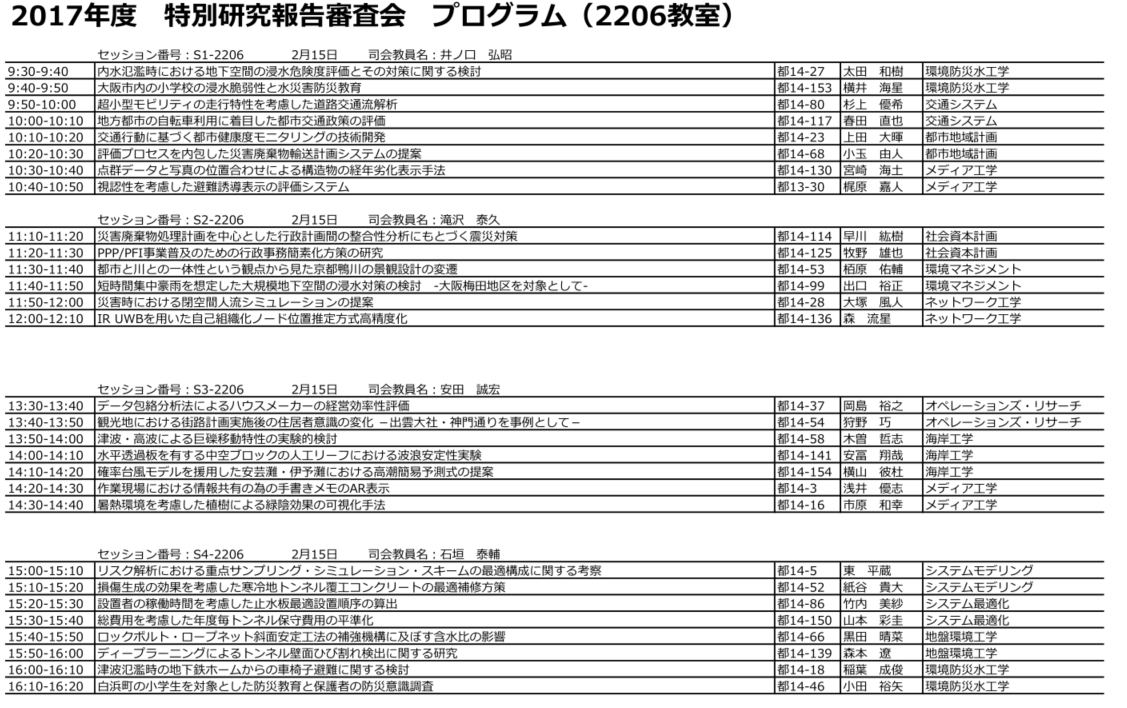
\includegraphics[scale=0.65]{t1.png}
    \caption{タイムテーブル $1/6$}
  \end{center}
\end{figure}

\begin{figure}[H]
  \begin{center}
    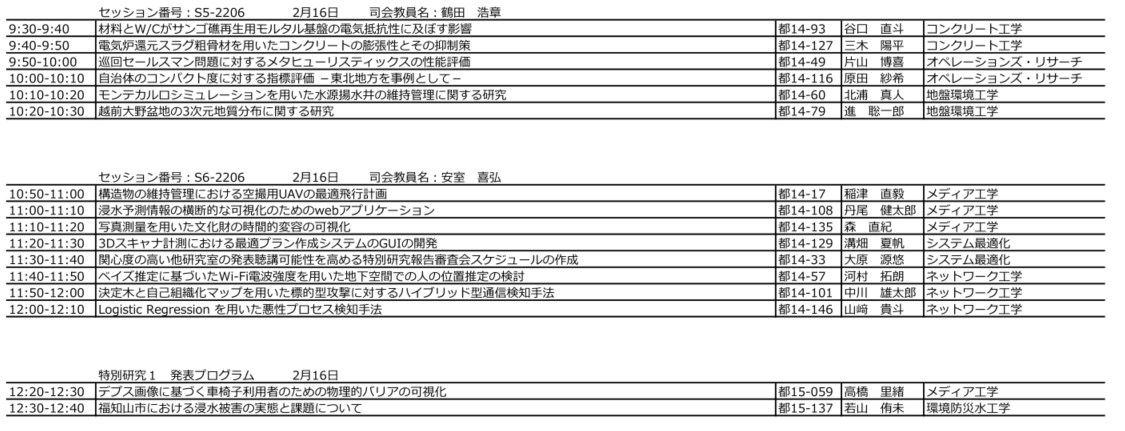
\includegraphics[scale=0.65]{t2.png}
    \caption{タイムテーブル $2/6$}
  \end{center}
\end{figure}

\begin{figure}[H]
  \begin{center}
    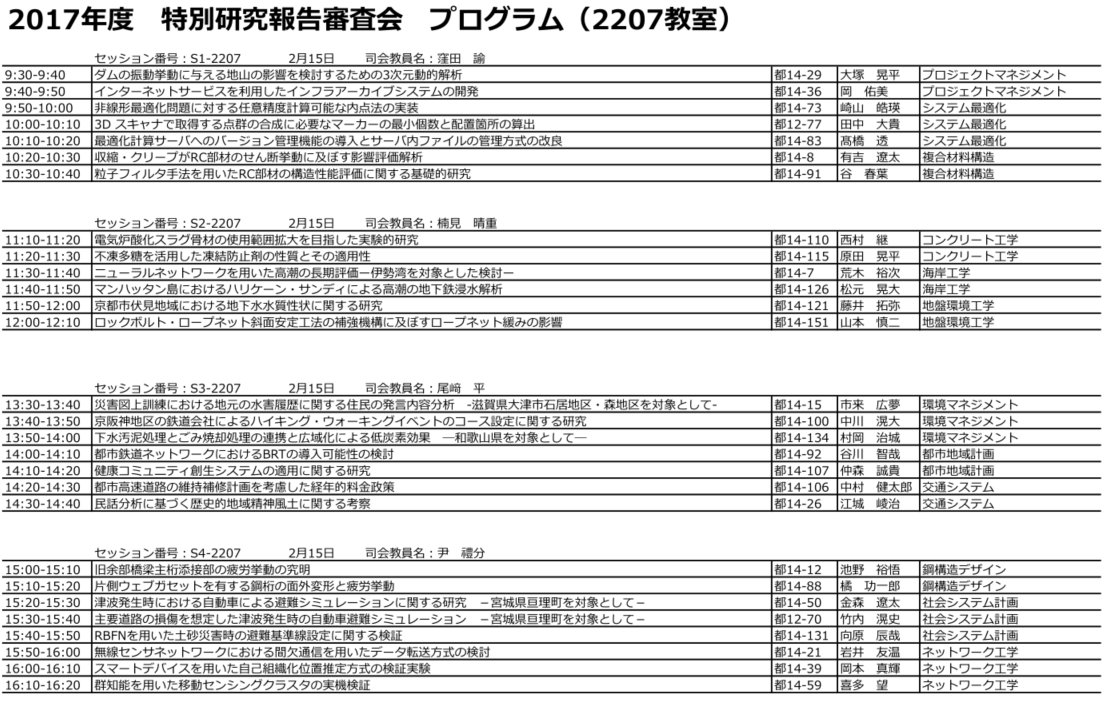
\includegraphics[scale=0.65]{t3.png}
    \caption{タイムテーブル $3/6$}
  \end{center}
\end{figure}

\begin{figure}[H]
  \begin{center}
    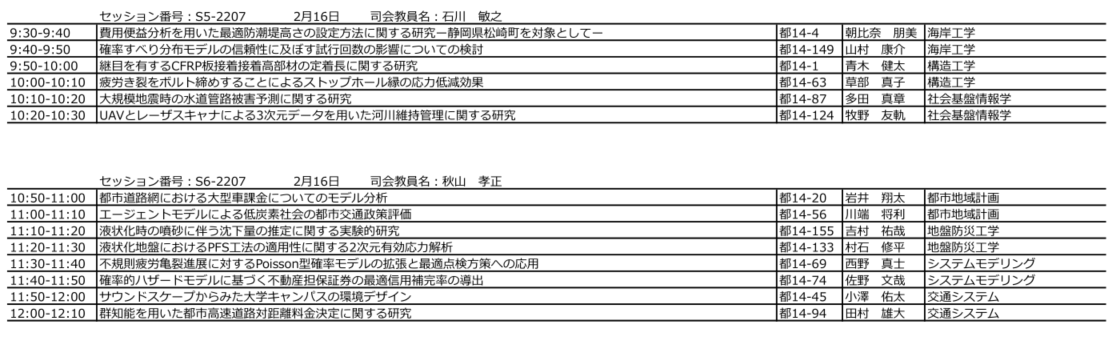
\includegraphics[scale=0.65]{t4.png}
    \caption{タイムテーブル $4/6$}
  \end{center}
\end{figure}

\begin{figure}[H]
  \begin{center}
    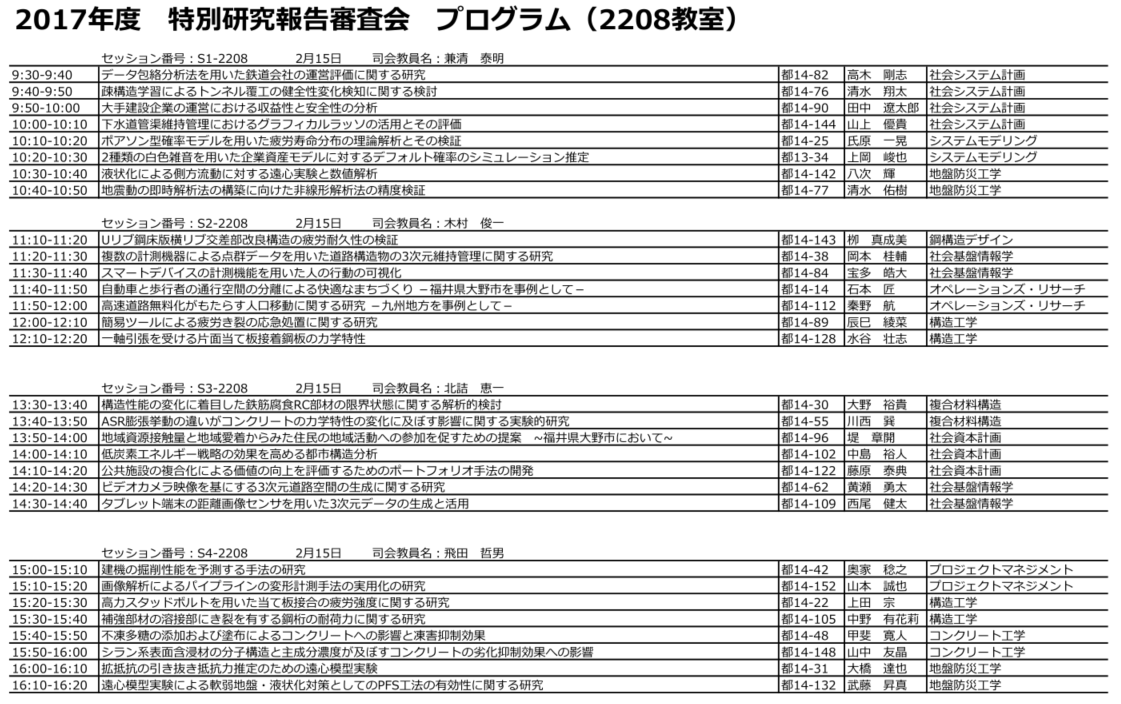
\includegraphics[scale=0.65]{t5.png}
    \caption{タイムテーブル $5/6$}
  \end{center}
\end{figure}

\begin{figure}[H]
  \begin{center}
    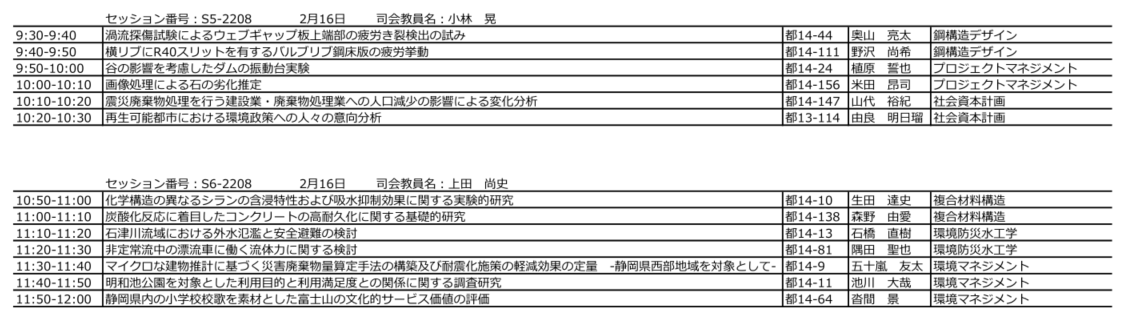
\includegraphics[scale=0.65]{t6.png}
    \caption{タイムテーブル $6/6$}
  \end{center}
\end{figure}

\begin{figure}[H]
  \begin{center}
    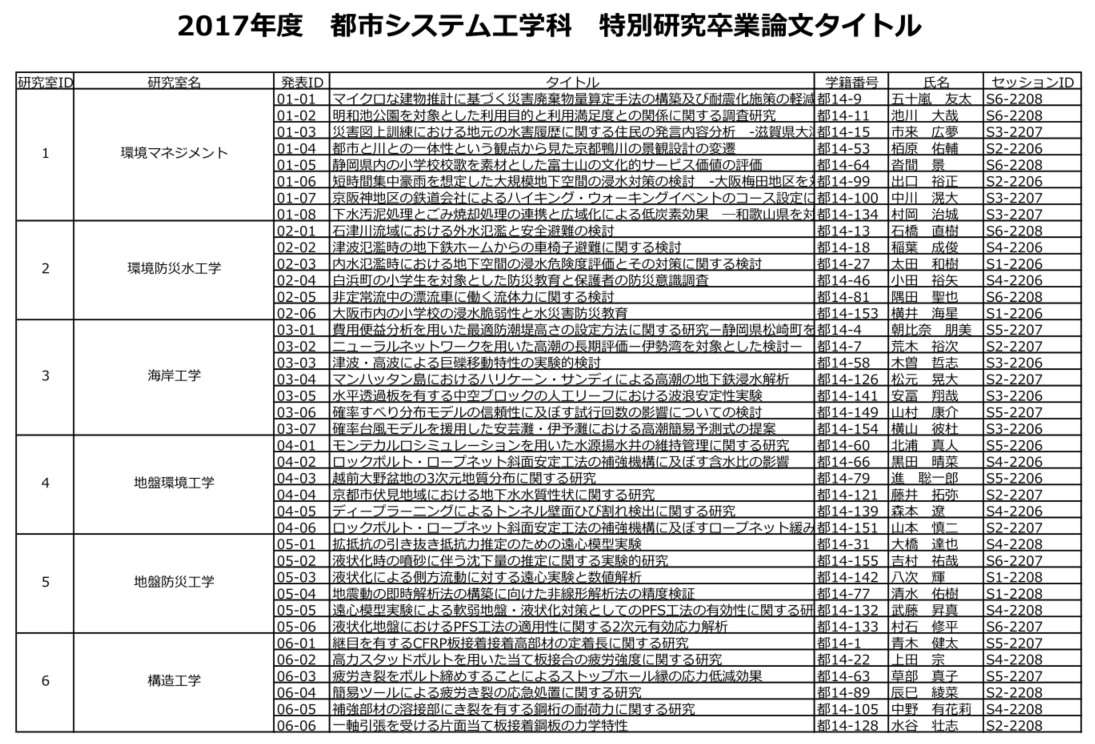
\includegraphics[scale=0.65]{ti3.png}
    \caption{タイトル一覧表 $1/4$}
  \end{center}
\end{figure}

\begin{figure}[H]
  \begin{center}
    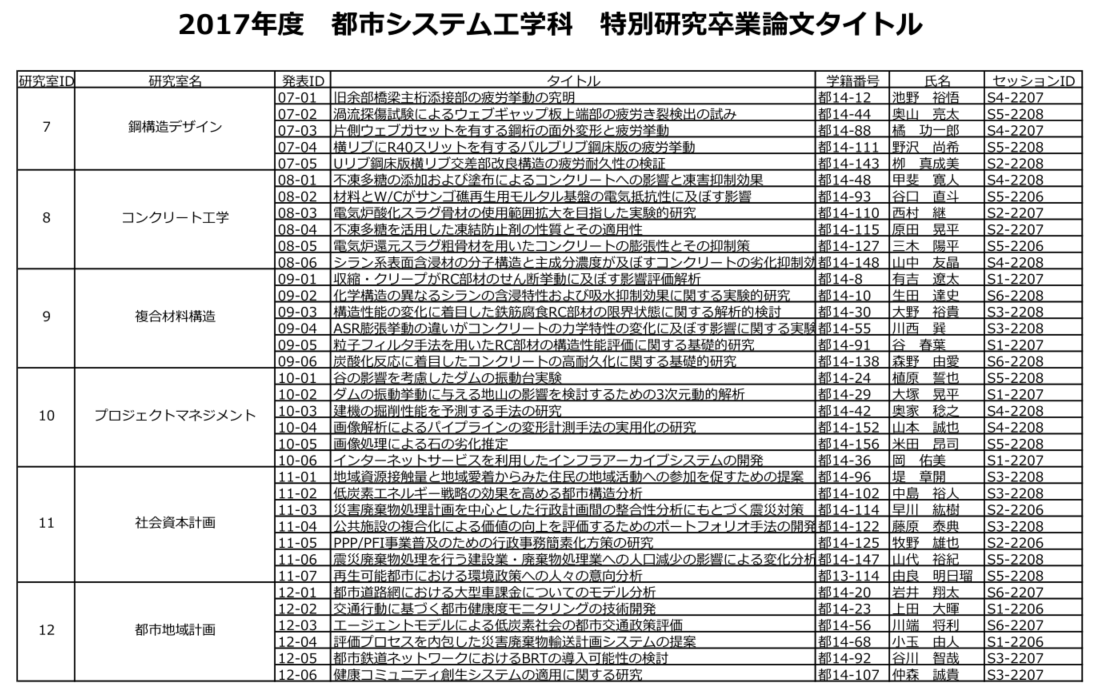
\includegraphics[scale=0.7]{ti4.png}
    \caption{タイトル一覧表 $2/4$}
  \end{center}
\end{figure}

\begin{figure}[H]
  \begin{center}
    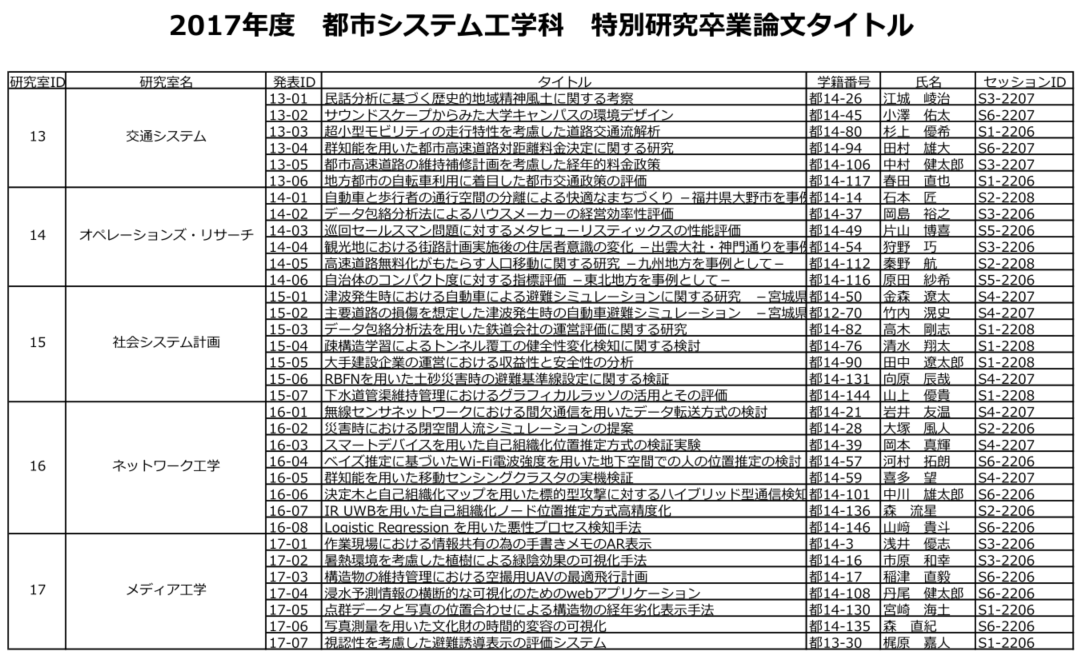
\includegraphics[scale=0.7]{ti1.png}
    \caption{タイトル一覧表 $3/4$}
  \end{center}
\end{figure}

\begin{figure}[H]
  \begin{center}
    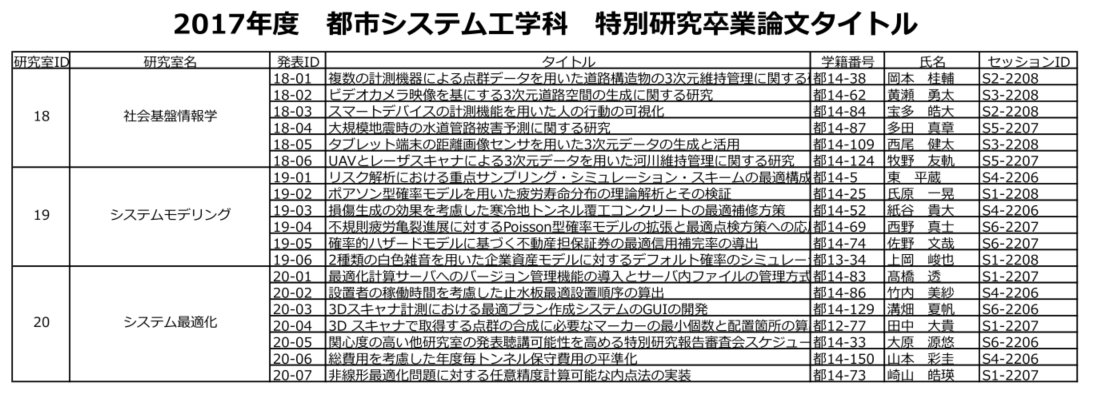
\includegraphics[scale=0.7]{ti2.png}
    \caption{タイトル一覧表 $4/4$}
  \end{center}
\end{figure}
%%%%%%%%%%%%%%%%%%%%%%%%%%%%%%%%%%%%%%%%%%%%%%%%%%%%%%%%%%%%%%%%%%%%%%
\end{document}
%%%%% End of file %%%%%
